\documentclass[review]{elsarticle}

\usepackage[margin=1in]{geometry}

\usepackage{lineno,hyperref}
\modulolinenumbers[5]

\usepackage{amsmath,amssymb,amstext} 
\usepackage{bm}
\usepackage{graphicx}
\usepackage{multirow}
\usepackage{empheq}
\usepackage{indentfirst}
\usepackage{natbib}
\usepackage{amsthm}

\newtheorem{thm}{Theorem} 
\newtheorem{lem}[thm]{Lemma} 
\newdefinition{rmk}{Remark} 
%\newproof{pf}{Proof}
%\newproof{pot}{Proof of (\ref{thm2})}

%\journal{Journal of \LaTeX\ Templates}

%%%%%%%%%%%%%%%%%%%%%%%
%% Elsevier bibliography styles
%%%%%%%%%%%%%%%%%%%%%%%
%% To change the style, put a % in front of the second line of the current style and
%% remove the % from the second line of the style you would like to use.
%%%%%%%%%%%%%%%%%%%%%%%

%% Numbered
%\bibliographystyle{model1-num-names}

%% Numbered without titles
%\bibliographystyle{model1a-num-names}

%% Harvard
%\bibliographystyle{model2-names.bst}\biboptions{authoryear}

%% Vancouver numbered
%\usepackage{numcompress}\bibliographystyle{model3-num-names}

%% Vancouver name/year
%\usepackage{numcompress}\bibliographystyle{model4-names}\biboptions{authoryear}

%% APA style
%\bibliographystyle{model5-names}\biboptions{authoryear}

%% AMA style
%\usepackage{numcompress}\bibliographystyle{model6-num-names}

%% `Elsevier LaTeX' style
\bibliographystyle{elsarticle-num}
%%%%%%%%%%%%%%%%%%%%%%%

\begin{document}

\begin{frontmatter}

%\title{Elsevier \LaTeX\ template\tnoteref{mytitlenote}}
%\tnotetext[mytitlenote]{Fully documented templates are available in the elsarticle package on \href{http://www.ctan.org/tex-archive/macros/latex/contrib/elsarticle}{CTAN}.}
\title{A semiparametric stochastic  mixed model for bivariate longitudinal data}


%% Group authors per affiliation:
\author{Kexin Ji
%\corref{mycorrespondingauthor} 
and Joel A. Dubin
%\fnref{myfootnote}
}
\address{Department of Statistics and Actuarial Science, University of Waterloo, 200 University Ave. W. Waterloo, Ontario N2L 3G1, Canada \\ 
kji@uwaterloo.ca, \ jdubin@uwaterloo.ca }
%\fntext[myfootnote]{Since 1880.}

% or include affiliations in footnotes:
%\author[mymainaddress,mysecondaryaddress]{Elsevier Inc}
%\ead[url]{www.elsevier.com}

%\author[mysecondaryaddress]{Global Customer Service\corref{mycorrespondingauthor}}
% \cortext[mycorrespondingauthor]{Corresponding author}
%\ead{kji@uwaterloo.ca}

%\address[mymainaddress]{1600 John F Kennedy Boulevard, Philadelphia}
%\address[mysecondaryaddress]{360 Park Avenue South, New York}

\begin{abstract}
We propose and consider inference for a semiparametric stochastic mixed model for bivariate longitudinal data. The approach models the mean of responses by parametric fixed effects and a smooth nonparametric function for the underlying time effects, and the relationship across the bivariate responses by a bivariate Gaussian random field and a joint distribution of random effects. 
The proposed model not only can model complicated individual hormone profiles, but also allows for more flexible within-subject and between-response correlations. 
The fixed effects regression coefficients and the nonparametric time functions are estimated using maximum penalized likelihood, where the resulting estimator for the nonparametric time function is a cubic smoothing spline. The smoothing parameters and all variance components are estimated simultaneously using restricted maximum likelihood.  Simulation results show that the parameter estimates are close to the true values with small standard errors. The fit of the proposed model on a real bivariate longitudinal dataset of pre-menopausal women performs well.
\end{abstract}

\begin{keyword}
Bivariate longitudinal data \sep Gaussian field \sep Penalized likelihood \sep Smoothing spline
% \MSC[2010] 00-01\sep  99-00
\end{keyword}

\end{frontmatter}

\linenumbers

%======================================================================
%
% S.1 INTRODUCTION
%
%
%======================================================================
\section{Introduction}

%Longitudinal data analysis has wide applications in areas such as medicine and agriculture. 
The distinctive feature of longitudinal data is that measurements of each subject are collected repeatedly over time, which induces a correlation structure among observations for the same subject. 
%Many methods have been developed over the years to accommodate this additional structure, e.g., \cite{Laird:1982}, \cite{Liang:1986}. 
For multivariate longitudinal data, repeated measurements are observed jointly for two or more responses. To better understand the relationships among the responses at the same time or different times, the correlation structure among the responses needs to be studied. 


The model we proposed is motivated by a longitudinal hormone study on estrogen and progesterone in pre-menopausal women, where assays of daily urine samples for metabolites of estrogen and progesterone are collected over one menstrual cycle. 
We are interested in modelling  time courses for the estrogen and progesterone metabolite profiles for a single cycle, the effects of covariates on the hormone excretion, and the potential correlation between the two hormones.  
Joint modeling of the hormone profiles of estrogen and progesterone is challenging.
First, the time courses of the univariate hormones profiles is complex such that
to model using a simple parametric function, such as linear mixed effects model, is insufficient; see Figure \ref{Liu1}. 
Second, multiple layers of correlation structures, say within-subject correlation between the bivariate hormones at different time points, also present a challenge.


\begin{figure}[h!]
\centering
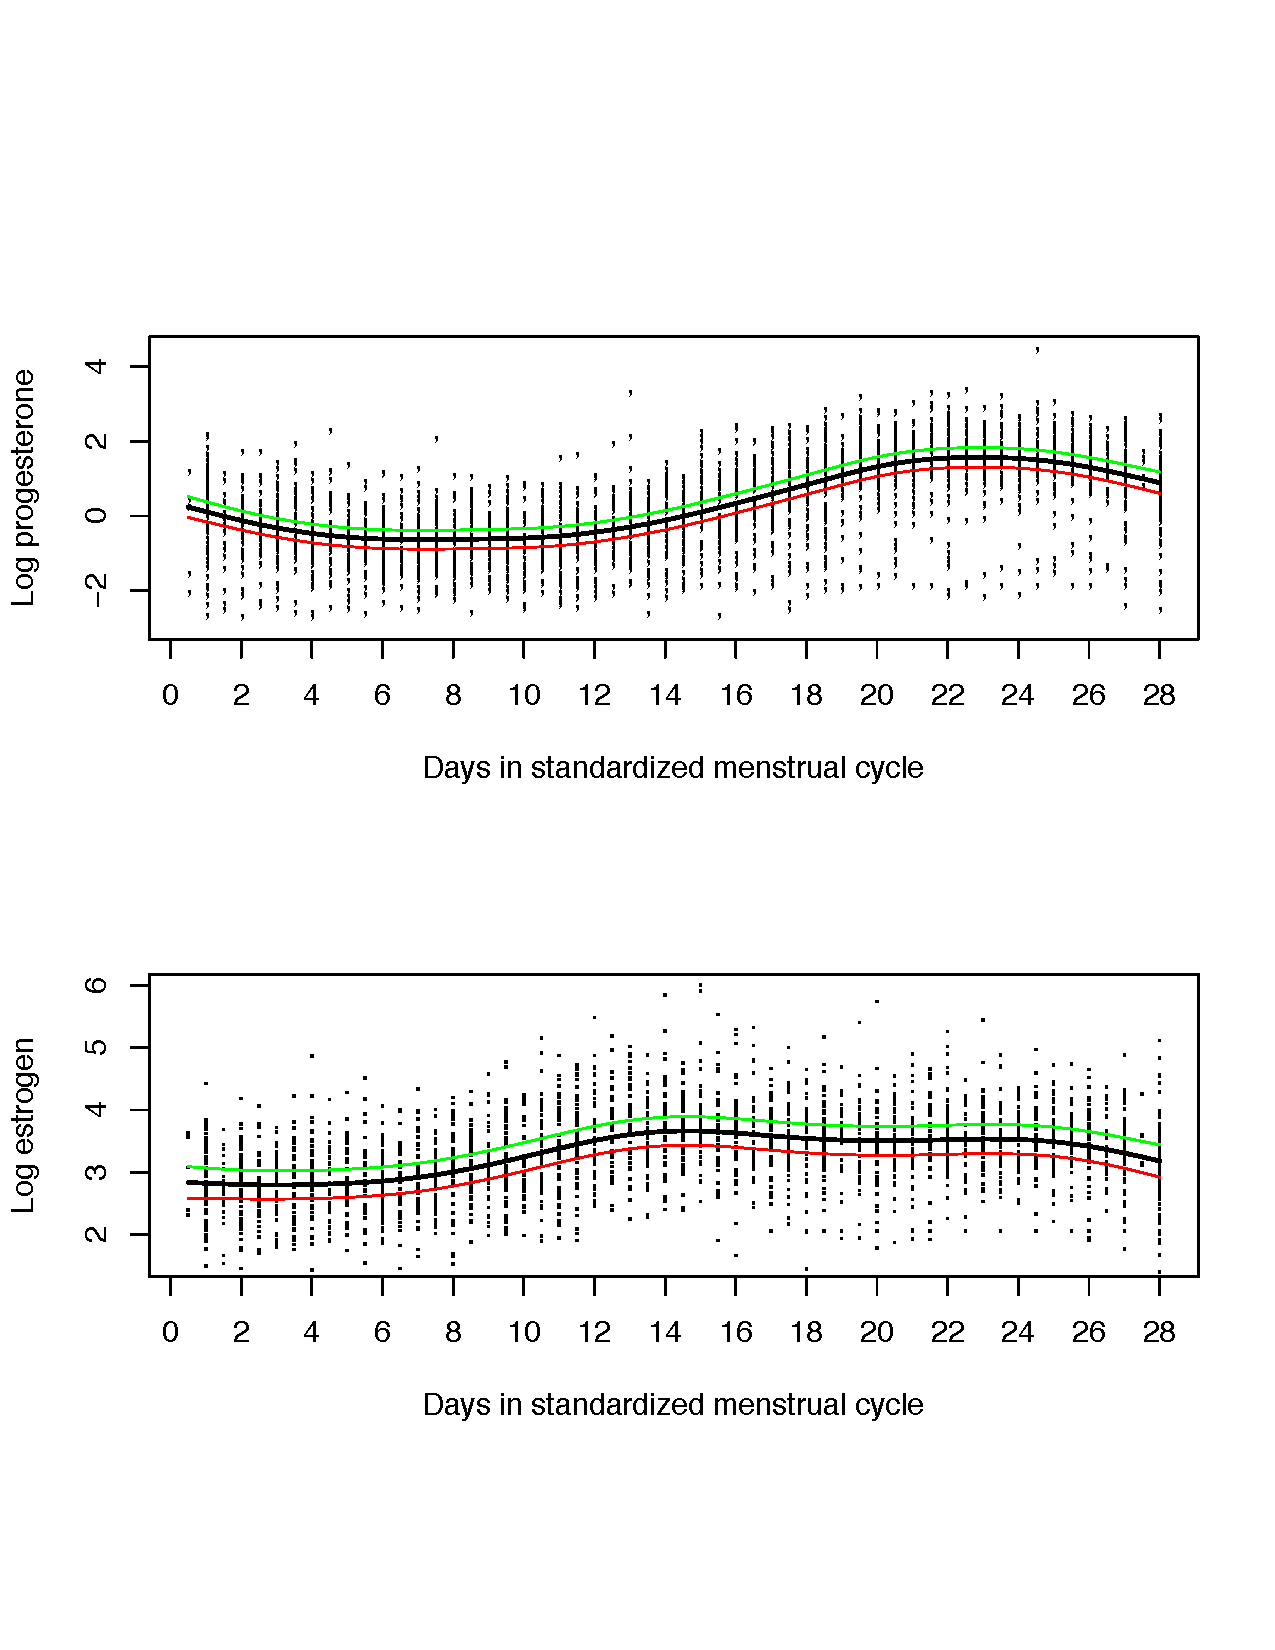
\includegraphics[width=0.7\textwidth]{bivLiuFig1.pdf}
\caption{Plots of log progesterone  and log estrogen levels against days in a standardized menstrual cycle, superimposed by estimated population mean curve $\hat f_1$ and $\hat f_2$.}
\label{Liu1}
\end{figure}

%Wide applications in areas such as medicine and agriculture require modelling longitudinal data to go beyond the usual linear mixed effects model, where the parametric assumptions are no longer sufficient.
% Beyond these earlier proposed models for linear and generalized linear longitudinal data, 
There have  been many extensions to allow for further flexibility in specifying the mean structure for  the modelling of  longitudinal data.  For example, 
\citet{Brumback:1998} used natural cubic splines to model the mean structure of the linear mixed model
%They extended the traditional LME  model to generalized smoothing spline models for samples of curves stratified by nested and crossed factors 
and specified the design matrices associated with fixed effects and random effects by bases of functions.
%, as opposed to the usual known covariates matrices.  
\citet{Verb:Cull:Kenw:Welh:quan:1999} 
used data-based determination of the smoothing parameters and applied to the analysis of designed experiments. 
Some efforts are also geared towards enriching the specifications of the correlation structure for the modelling of longitudinal data.
\citet{Tayl:Cumb:Sy:quan:1994} used an integrated Ornstein-Uhlenbeck process to model the covariance structure.
 \cite {Zhang:1998} and \citet{Zhan:Lin:Sowe:quan:2000}  proposed a  semiparametric stochastic mixed model for regular and periodic longitudinal data, respectively, where   covariate effects are modelled parametrically and the underlying complex (periodic) time courses are modelled nonparametrically; and used a stochastic process and random effects to model the within-subject and between-subject correlation respectively. 
Instead of  smoothing splines, \cite{Welh:Cull:Kenw:Thom:quan:2006} modelled cyclic longitudinal data using mixed model L-splines. 
%Meyer et al \cite{meyer} proposed a functional data analysis approach to model cyclic data. 
\citet{Wood:2006} used a penalized cubic regression spline to model a cyclic smooth function. 
These models, however at this stage to our knowledge, are only applicable to univariate longitudinal analysis.


Some of the univariate techniques have been extended to the multivariate case.
For example, 
\citet{Sy:Cumb:Tayl:quan:1997} employed multivariate stochastic processes to jointly model  bivariate longitudinal data. 
 More recently, \cite{Raffa:2015} modelled bivariate longitudinal responses, from outcomes of different data types, via a mixed effects hidden Markov modeling approach.  And, most relevant in terms of the type of data focused upon in this paper,  \cite{Liu:Capp:Crof:Guo:quan:2014} extended the univariate state space model in time series analysis, and proposed a bivariate hierarchical state space model to bivariate circadian rhythmic  longitudinal responses;
each response is modelled by a hierarchical state space model, with both population-average and subject-specific components; and the bivariate model is constructed by linking the univariate models based on the hypothesized relationship between the responses. 

In the current paper, we extend \citet {Zhang:1998} and propose a bivariate semiparametric stochastic mixed model for bivariate repeated measures data.  The bivariate model uses parametric fixed effects and smooth nonparametric functions for each of the two underlying time effects. 
The between-subject correlations are modelled using separate but correlated random effects and the within-subject correlations by a bivariate Gaussian random field. 
The model allows us to investigate the relationship of the two responses through the correlation of the random effects and the bivariate Gaussian fields, which can not only describe the concurrent relationship of the two responses but also allows for characterizations of the relationship across time points.
We derive maximum penalized likelihood estimators for both the fixed effects regression coefficients and the nonparametric time functions. The smoothing parameters and all variance components are estimated simultaneously using restricted maximum likelihood.  


The paper is organized as followed. Section \ref{modelSpe} specifies the proposed model with assumptions. Section \ref{est} provides estimation and inference procedures. Specifically, Sections \ref{estimation} gives estimation procedures for  the model parameters, the nonparametric components, random effects and the Gaussian fields.  
Section \ref{biasCov} specifies the biases and covariances for all the estimators given in Section \ref{estimation}; and Section \ref{estSmoo}  concludes this section by providing the estimation procedures of the smoothing parameters and variance components. 
Section \ref{simulation} investigates the proposed methodology through a simulation study.  
Section \ref{dataAnalysis}  illustrates the model by analyzing bivariate longitudinal female hormone data collected daily over a single menstrual cycle, and finally, Section \ref{discu} provides a summary of our proposed model, and discusses challenges and future work. 
%Technical details are included in Appendix \ref{}.

%======================================================================
%
% S.2 MODEL SPECIFICATION
%
%
%======================================================================
\section{The Bivariate Semiparametric Stochastic Mixed Effects Model} \label{modelSpe}


%---------------------------------------------------------------------------------------------------------------------------
\subsection{The Proposed Model Specifications and Assumptions}
Denote $\bm Y_{ij} = (Y_{1ij}, Y_{2ij})^T$ to be the bivariate metabolite levels of estrogen and progesterone for the $i$th subject at time point $t_{ij}$, 
$i = 1, \dots, m$ and $j = 1, \dots, n_i$. 
The bivariate model is
\begin{equation} \label{biv}
\boldsymbol Y_{ij} 
=
\boldsymbol X_{ij}^T\boldsymbol{\beta} +
\boldsymbol f(t_{ij}) + \boldsymbol Z_{ij}^T
\boldsymbol b_{i} + 
\boldsymbol U_{i}(t_{ij}) + 
\boldsymbol \epsilon_{ij},
\end{equation}
where 
$\bm \beta = (\bm \beta_1, \bm \beta_2)^T$ are $(p_1 +p_2) \times 1$ vectors of fixed effects regression coefficients associated with known covariates $\bm X_{ij}={\rm diag}(\bm X_{1ij}^T, \bm X_{2ij}^T)$; 
$\bm b = (\bm b_{1i}, \bm b_{2i})^T$ are $2q \times 1$ vectors of random effects, respectively, associated with known covariates $\bm Z_{ij}={\rm diag}(\bm Z_{1ij}^T, \bm Z_{2ij}^T)$; 
$\bm f(t) = (f_1(t), f_2(t))^T$ are  twice-differentiable  smooth functions of time; 
$\bm U_i(t) = (U_{1i}(t), U_{2i}(t))^T$ is a mean zero bivariate Gaussian field  with 
covariance matrix 
%%\E\{((U_i(s))^\prime U_i(t)\} =
\begin{eqnarray} \label{gfcov}
\boldsymbol C_i(s, t) &=&
%  \begin{pmatrix}
%  E[U_{i1}(s) U_{i1}(t)] &  E[U_{i1}(s) U_{i2}(t)]   \\
%E[U_{i2}(s) U_{i1}(t)]  &   E[U_{i2}(s) U_{i2}(t)]  
% \end{pmatrix} \\ 
%&=&
  \begin{pmatrix}
 \sqrt {\xi_1(s) \xi_1(t)} \eta_1(\rho_1; s, t) &   \sqrt {\xi_1(s) \xi_2(t)} \eta_3(\rho_3; s, t)
  \\
 \sqrt {\xi_2(s) \xi_1(t)} \eta_3(\rho_3; t, s)
 &   \sqrt {\xi_2(s) \xi_2(t)} \eta_2(\rho_2; s, t)
 \end{pmatrix}
\end{eqnarray}
%$$
%C_{ij}(s, t) = \E\{((U_i(s))^\prime U_i(t)\}
%$$
%both mean-zero Gaussian processes with
where 
$\xi_1(t)$ and $\xi_2(t)$ are  variance functions;  
${\rm corr} (U_{1i}(t), U_{1i}(s)) = \eta_1(\rho_1; s, t)$,  \\
${\rm corr} (U_{2i}(t), U_{2i}(s)) = \eta_2(\rho_2; s, t)$, 
and ${\rm corr} (U_{1i}(t), U_{2i}(s)) = \eta_3(\rho_3; s, t)$
 are correlation functions, where 
% $\rho_1 \in [0, 1]$,  $\rho_2 \in [0, 1]$ and $\rho_3 \in [0, 1]$ 
$\rho_1$,  $\rho_2$ and $\rho_3$ 
are correlation coefficients; 
and 
the measurement errors $\epsilon_{ij} = (\epsilon_{1ij}, \epsilon_{2ij})^T$ are bivariate  normal with mean $\bm 0$ and variance ${\rm diag}(\sigma_1^2, \sigma_2^2)$.
We assume  $\bm b_i$ to be  $2q$-dimensional normal  with mean zero and unstructured covariance matrix $\bm G(\bm \phi)$,   
% These random effects, $\bm b_{1i}$ and $\bm b_{2i}$, are assumed to be separate but correlated. 
and that the random effects, the stochastic process and the measurement error to be mutually independent. 

This model (\ref{biv}) is an extension to the model proposed in \citet {Zhang:1998}, where a univariate semiparametric stochastic mixed model for longitudinal data was proposed. The challenge here is that we are modeling a bivariate longitudinal response model, which  is achieved  by modeling a joint distribution of the random effects and the bivariate Gaussian field. The distributions of the two random effects can be potentially distinct, with different distributions or the same distribution with different parameters; but the two random effects are  assumed separate but correlated. 

%---------------------------------------------------------------------------------------------------------------------------
\subsection{Matrix Notation} \label{MatrixNotation}

To make inferences from the model (\ref{biv}), we will  write the model in matrix form -  first, in subject level; then, over all subjects.  

Denote $\bm Y_{i} = (\bm Y_{i1}, \dots, \bm Y_{in_i})^T$ and similarly for $\bm X_i$, $\bm Z_i$, $\bm U_i$ and $\bm \epsilon_i$. 
Let 
 $
\bm t^\prime = (t_{1}^\prime, \dots, t_r^\prime)
 $
be a vector of ordered distinct values of $t_{ij}, i = 1, \dots, m$ and $j = 1\dots n_i$ and
define
 $\bm {\tilde N}_i$ to be the $n_i \times r$ incidence matrix for the $i^{\rm th}$ subject connecting 
 $
 \bm t_i = (t_{i1}, \dots, t_{in_i})^T 
 $
 and
 $\bm t^\prime$ such that
 $$
\bm {\tilde N}_i [j, \ell] =
\begin{cases}
1 & \text{if } t_{ij}^\prime = t_\ell^\prime \\
0 & \text{otherwise},
\end{cases}
$$
where 
$\bm {\tilde N}_i [j, \ell]$ denotes the $(j, \ell)^{\rm th}$ entry of matrix $\bm {\tilde N}_i$ for $j = 1, \dots, n_i$ and $\ell = 1, \dots, r_1$. 
Let $\boldsymbol N_{1i} = \boldsymbol A_{1i} \boldsymbol {\tilde N} _i$  and $\boldsymbol N_{2i} = \boldsymbol A_{2i} \boldsymbol {\tilde N}_i$,  be the incidence matrices for the first and second response,
respectively, where 
\[
\boldsymbol A_{1i} =
 \begin{pmatrix}
   1 & 0 & 0 &  \dots & 0 \\
  0 & 0 & 0 &   \dots & 0 \\
  0 & 1 & 0 & \dots & 0 \\
   0 & 0 & 0 &   \dots & 0  \\
  \vdots &  & \ddots &  \\ 
 0 & \dots & 0  & 0 & 1\\
  0 & 0 & 0 &   \dots & 0 \\
 \end{pmatrix}
   \in {\rm I\!R}^{2n_i \times n_i},
\quad
\boldsymbol A_{2i} =
  \begin{pmatrix}
 0 & 0 & 0 &   \dots & 0 \\
1 & 0 & 0 &  \dots & 0 \\
 0 & 0 & 0 &   \dots & 0\\
0 & 1 & 0 & \dots & 0\\
  \vdots &  & \ddots &  \\ 
0 & 0 & 0 &   \dots & 0\\
0 & \dots & 0  & 0 & 1 \\
 \end{pmatrix}
  \in {\rm I\!R}^{2n_i \times n_i}.
 \]
Then, the proposed bivariate semiparametric stochastic mixed model  (\ref{biv}) can be written as
$$
\boldsymbol Y_{i} 
=
\boldsymbol{X_{i}}\boldsymbol{\beta} +
 \boldsymbol N_{1i} \boldsymbol f_1 + 
  \boldsymbol N_{2i} \boldsymbol f_2 + 
\boldsymbol{Z_{i}}\boldsymbol{b_{i}} + 
\boldsymbol U_{i} + 
\boldsymbol \epsilon_{i}
$$
for subject $i$, where 
$\bm f_1 = (f_1(t_1^\prime), \dots, f_1(t_r^\prime))^T$
and 
$\bm f_2 = (f_2(t_1^\prime), \dots, f_2(t_r^\prime))^T$.
Note that here we implicitly assume that each subject has distinct and potentially unequally spaced time points and that the bivariate responses are observed at the same time point for the same subject which is often realized in actual data applications, though this assumption can be easily modified if needed.

Further denoting $\boldsymbol  Y = (\boldsymbol Y_1^T, \dots, \boldsymbol Y_m^T)^T$ and $\boldsymbol  X$, $\boldsymbol  N_1$, $\boldsymbol  N_2, \boldsymbol b, \boldsymbol U, \boldsymbol \epsilon$ similarly and letting $n = \sum_{i = 1}^m n_i$, then  the bivariate semiparametric stochastic mixed effects model over all subjects is 
\begin{equation} \label{propM}
\boldsymbol Y 
=
\boldsymbol{X}\boldsymbol{\beta} 
+ \boldsymbol N_1 \boldsymbol f_1 
+ \boldsymbol N_2 \boldsymbol f_2 
+ \boldsymbol{Z}\boldsymbol{b}
+ \boldsymbol U 
+ \boldsymbol \epsilon,
\end{equation}
with assumptions 
\[
 \begin{pmatrix}
  \boldsymbol b \\
  \boldsymbol U  \\
 \boldsymbol \epsilon
 \end{pmatrix}
 \sim 
 \boldsymbol N \left(
 \begin{pmatrix}
\boldsymbol 0 \\
\boldsymbol 0 \\
 \boldsymbol 0 
 \end{pmatrix},
  \begin{pmatrix}
  \boldsymbol D(\boldsymbol \phi) &  \boldsymbol 0 & 0 \\
  \boldsymbol 0 & \boldsymbol \Gamma (\boldsymbol \xi, \rho) & \boldsymbol 0 \\
 \boldsymbol 0 & \boldsymbol 0 &  \boldsymbol \Sigma (\boldsymbol \sigma^2) 
 \end{pmatrix}
 \right) 
\]
where 
% b
$\boldsymbol D (\boldsymbol \phi) = {\rm diag} (\boldsymbol G, \dots, \boldsymbol G)$; 
% U
$\boldsymbol \Gamma (\boldsymbol \xi, \rho) = {\rm diag} (  \boldsymbol \Gamma_1 (\boldsymbol t_1, \boldsymbol t_1), \dots,   \boldsymbol \Gamma_m(\boldsymbol t_m, \boldsymbol t_m))$
and the $(k, k^\prime)^{\rm th}$ entry of $ \boldsymbol \Gamma_i(\boldsymbol t_i, \boldsymbol t_i)$ is $\boldsymbol C_i(k, k^\prime)$;
% eps
and $\bm \Sigma(\bm \sigma^2)$ is the diagonal matrix with alternating entries $\sigma^2_1$ and $\sigma^2_2$. 

%---------------------------------------------------------------------------------------------------------------------------
\subsection{Covariance Structures} \label{bivRes}


%The proposed model (\ref{propM}) can also be rewritten as a {\it three-level hierarchical model}
%\begin{eqnarray}
%% CONDITIONAL MODEL
%\boldsymbol Y| \boldsymbol b, \boldsymbol U 
%&\sim&
%N_{2n} \left(\boldsymbol{X}\boldsymbol{\beta} +
% \boldsymbol N_{1} \boldsymbol f_1 + 
%  \boldsymbol N_{2} \boldsymbol f_2 + 
%\boldsymbol{Z}\boldsymbol{b} + \boldsymbol U,  
%\boldsymbol \Sigma \right)
%\label{condM}
%\\ 
%% DISTRIBUTION OF b
%\boldsymbol b &\sim& N_{2m} (\boldsymbol 0, \boldsymbol D)   
%\label{bDis} 
%\\
%% DISTRIBUTION OF U
%\boldsymbol U &\sim& N_{2n} (\boldsymbol 0, \boldsymbol \Gamma); \label{uDis} 
%\end{eqnarray}

(a) Mean and Covariance of the Proposed Model

The marginal  or population-averaged mean of $\bm Y$ is 
$$
E(\bm Y) = \bm X \bm \beta + \bm N_1 \bm f_1 + \bm N_2 \bm f_2,
$$
and the marginal covariance of $\bm Y$, averaged over the distribution of subject-specific effects $\bm b$ is
$$
{\rm cov}(\bm Y) = \bm Z \bm D \bm Z^T + \bm \Gamma + \bm \Sigma.
$$
% which account for the correlation among the repeated observations on the same individuals in a longitudinal study.
The mean response for a specific subject is 
$$
E(\bm Y | \bm b) = \bm X \bm \beta + \bm N_1 \bm f_1 + \bm N_2 \bm f_2 + \bm Z \bm b, 
$$
and the covariance among the longitudinal observations for a specific subject is
$$
{\rm cov}(\bm Y | \bm b) = {\rm cov}(\bm U) + {\rm cov}(\bm \epsilon) = \bm \Gamma + \bm \Sigma,
$$
which describes the covariance of the subject deviations from the subject-specific mean response $E(\bm Y | \bm b)$.
The within-subject correlation ($\bm \Gamma + \bm \Sigma$) structure is enhanced by the addition of  bivariate Gaussian field into the model.

(b) Modelling the Relationship of the Bivariate Responses

Moreover, the proposed model also allows for explicit analysis of the relationship of the bivariate responses, which is explained by the covariance of the random effects and and the covariance of the bivariate Gaussian field. 
Specifically, the covariance between the bivariate responses at time points $t_{ij}$ and $t_{ik}$ for individual $i$ is given by
\begin{eqnarray*}
&&
{\rm cov}(Y_{1ij}, Y_{2ik}) \\&=& 
{\rm cov}(\bm {X_{1ij}}^T\bm{\beta_1} + f_1(t_{ij}) 
+ \bm{Z_{1ij}}^T\bm{b_{1i}} + U_{1i}(t_{ij}) + \epsilon_{1ij}, 
% && \quad\quad
\bm{X_{2ik}}^T\bm{\beta_2} + f_2(t_{ik}) + \bm{Z_{2ik}}^T\bm{b_{2i}} + 
U_{2i}(t_{ik}) + \epsilon_{2ik}) \\
&=& {\rm cov} (\bm{Z_{1ij}}^T\bm{b_{1i}} + U_{1i}(t_{ij}) + \epsilon_{1ij},
\bm{Z_{2ik}}^T\bm{b_{2i}} + U_{2i}(t_{ik}) + \epsilon_{2ik}) \\
&=& \bm{Z_{1ij}}^T {\rm cov} (\bm{b_{1i}}, \bm{b_{2i}})\bm{Z_{2ik}}
+ {\rm cov}(U_{1i}(t_{ij}), U_{2i}(t_{ik})) \\
% + {\rm cov}(\epsilon_{1ij}, \epsilon_{2ik}) \\ 
&=&
\bm{Z_{1ij}}^T \bm G^\prime \bm{Z_{2ik}}
+  \sqrt {\xi_1(t_{ij}) \xi_2(t_{ik})} \eta_3(\rho_3; t_{ij}, t_{ik}),
\end{eqnarray*}
where $\bm G^\prime$ is the $q$ by $q$ upper off-diagonal block matrix of covariance matrix $\bm G$ for the random effects $\bm b_i$. 
The result shows that the inclusion of bivariate Gaussian field  allows for modelling the covariance of the bivariate responses at different time points.

%---------------------------------------------------------------------------------------------------------------------------
\subsection{The Gaussian Field Specification}

To accommodate for more complicated within-subject correlation and potential correlation between the bivariate responses, we propose to include various stationary and nonstationary bivariate Gaussian fields to model serial correlation. This allows for the within-subject covariance and the correlation between bivariate responses to be a function of time. 

There are potentially many choices available: Wiener process or Brownian motion \citep{Tayl:Cumb:Sy:quan:1994}; an integrated Wiener process and so on. One particular Gaussian process/field worthy of mentioning is the Ornstein-Uhlenbeck (OU) process \citep{Koralov:2007} which has a correlation function that decays exponentially over time corr($U_i(t), U_i(s)$) = $\exp\{-\alpha|s-t|\}$. The variance function for OU process $\xi(t) = \sigma^2/2a$ is a constant, thus the process is strictly stationary. When $\xi(t)$ varies over time, then the process becomes nonhomogenesous (NOU) and, for example, we can assume $\xi(t) = \exp(a_0 + a_1 t + a_1 t^2)$. 

%======================================================================
%
% S.3 ESTIMATION
%
%
%======================================================================
\section{Estimation and Inference} \label{est}


%---------------------------------------------------------------------------------------------------------------------------
\subsection{Estimation of Model Coefficients, Nonparametric Function, Random Effects and Gaussian Fields} \label{estimation}

The proposed model (\ref{propM})  implies the {\it marginal model}
\[
% \begin{equation}\label{marginal}
%  MARGINAL MODEL
Y = \boldsymbol{X}\boldsymbol{\beta} +
 \boldsymbol N_{1} \boldsymbol f_1 + 
  \boldsymbol N_{2} \boldsymbol f_2 + \boldsymbol \epsilon^*,   
% DISTRIBUTION OF epsilon*
\boldsymbol \epsilon^* \sim N_{2n}(\boldsymbol 0, \boldsymbol V) 
% \end{equation}
\]
where $\boldsymbol V = \boldsymbol  Z  \boldsymbol D  \boldsymbol Z^T
  +  \boldsymbol  \Gamma
  +   \boldsymbol \Sigma$.
  Thus, the {\it log-likelihood} function for 
$(\boldsymbol \beta, \boldsymbol f_1, \boldsymbol f_2)$  is :
\begin{eqnarray*}
&& 
\ell (\boldsymbol \beta, \boldsymbol f_1, \boldsymbol f_2; \boldsymbol Y)
\propto
-{1 \over 2} \log |\boldsymbol V| 
 -{1 \over 2}
 (\boldsymbol Y - \boldsymbol\beta 
 - \boldsymbol N_1 \boldsymbol f_1 - \boldsymbol N_2 \boldsymbol f_2)^T 
 \boldsymbol V^{-1} 
  (\boldsymbol Y - \boldsymbol\beta  
  - \boldsymbol N_1 \boldsymbol f_1 - \boldsymbol N_2 \boldsymbol f_2)
\end{eqnarray*}
for given fixed variance parameters.
We   estimate the parameters $\boldsymbol \beta$, $\boldsymbol f_1$ and $\boldsymbol f_2$ by  maximizing  the penalized likelihood \citep*{Wang:Guo:Brow:quan:2000}:
\begin{equation} \label{penLog}
\ell(\mbox{\boldmath$\beta$}, \boldsymbol f_1, \boldsymbol f_2 ; \boldsymbol Y) 
 - \lambda_1\int_a^b [f_1^{\prime\prime}(t)]^2 dt  
 - \lambda_2 \int_a^b [f_2^{\prime\prime}(t)]^2 dt 
= 
\ell(\mbox{\boldmath$\beta$}, \boldsymbol f_1, \boldsymbol f_2 ; \boldsymbol Y) 
- \lambda_1
\boldsymbol f_1^T \boldsymbol K \boldsymbol f_1
 - \lambda_2
\boldsymbol f_2^T \boldsymbol K \boldsymbol f_2 
\end{equation}
where 
$\lambda_1$ and $\lambda_2$ are smoothing parameters; 
$a$ and $b$ is the range of time $t$; and 
$\boldsymbol K$ is the nonnegative definite smoothing matrix, defined in Equation (2.3) in \citet{Green:1994}. 
Since observation time points $t_{ij}$ are assumed to be the same for both responses, the smoothing matrix $\bm K$, which is determined by time increments, is also the same.
The resulting estimators for the nonparametric functions  are  the natural cubic spline estimators  of $\boldsymbol f_1$ and $\boldsymbol f_2$. 

% DIFFERENTIATION
Differentiation of (\ref{penLog}) with respect to $\boldsymbol \beta$, $\boldsymbol f_1$, $\boldsymbol f_2$ gives the estimators 
$(\boldsymbol {\hat \beta}, \boldsymbol {\hat f}_1, \boldsymbol {\hat f}_2)$ that solves
\begin{equation} \label{normalMatrix}
 \begin{pmatrix}
  \boldsymbol X^T  \boldsymbol W \boldsymbol X & \boldsymbol X^T  \boldsymbol W \boldsymbol N_1 & \boldsymbol X^T  \boldsymbol W \boldsymbol N_2 \\
   \boldsymbol N_1^T  \boldsymbol W\boldsymbol X & \boldsymbol N_1^T  \boldsymbol W \boldsymbol N_1 \boldsymbol 
 + \lambda_1 \boldsymbol K &  \boldsymbol N_1^T  \boldsymbol W \boldsymbol N_2  \\
  \boldsymbol N_2^T  \boldsymbol W\boldsymbol X &  \boldsymbol N_2^T  \boldsymbol W \boldsymbol N_1 & \boldsymbol N_2^T  \boldsymbol W \boldsymbol N_2 \boldsymbol 
 +
  \lambda_2 \boldsymbol K \\
 \end{pmatrix}
  \begin{pmatrix}
   \boldsymbol \beta \\
 \boldsymbol f_1 \\
 \boldsymbol f_2\\
 \end{pmatrix}
  =
 \begin{pmatrix}
   \boldsymbol X^T  \boldsymbol W \boldsymbol Y \\
   \boldsymbol N_1^T  \boldsymbol W \boldsymbol Y  \\
  \boldsymbol N_2^T  \boldsymbol W \boldsymbol Y  \\
 \end{pmatrix},
 \end{equation}
where $\boldsymbol W = \boldsymbol V^{-1}$.
% CLOSED-FORM SOL'N
To study the theoretical properties of the estimates, such as bias and covariance, we derive the closed-form solutions  for $\boldsymbol {\hat \beta}$, $\boldsymbol {\hat f}_1$ and $\boldsymbol {\hat f}_2$
\begin{eqnarray}
 % ESTIMATE FOR BETA
 \boldsymbol {\hat \beta} 
  &=&
 (\boldsymbol X^T  \boldsymbol W_x \boldsymbol X )^{-1} \boldsymbol X^T  \boldsymbol W_x \boldsymbol Y 
\label{betaHat} \\
% ESTIMATE FOR F_1
 \boldsymbol {\hat f}_1
   &=&
  (\boldsymbol N_1^T 
\boldsymbol W_{f_1}  \boldsymbol N_1
  + \lambda_1 \boldsymbol K)^{-1}  \boldsymbol N_1^T \boldsymbol W_{f_1} \boldsymbol Y
\label{f1Hat} \\
% ESTIMATE FOR F_2
  \boldsymbol {\hat f}_2 
  &=&
 (\boldsymbol N_2^T 
\boldsymbol W_{f_2}  \boldsymbol N_2
  + \lambda_2 \boldsymbol K)^{-1}  \boldsymbol N_2^T \boldsymbol W_{f_2} \boldsymbol Y,
\label{f2Hat}
\end{eqnarray}
% WEIGHT MATRICES
where 
     % W_x
$ \boldsymbol W_x =
 \boldsymbol W_1 
 -
\boldsymbol W_1 \boldsymbol N_2 
 (\boldsymbol N_2^T  \boldsymbol W_1 \boldsymbol N_2 \boldsymbol 
 + \lambda_2 \boldsymbol K)^{-1} 
 \boldsymbol N_2^T  \boldsymbol W_1$, 
     % W_f1
 $\boldsymbol W_{f_1}  =  \boldsymbol W_2 - \boldsymbol W_2\boldsymbol X(\boldsymbol X^T  \boldsymbol W_2\boldsymbol X)^{-1}  \boldsymbol X^T  \boldsymbol W_2,$
 and 
      % W_f2
 $\boldsymbol W_{f_2}  =  \boldsymbol W_1 - \boldsymbol W_1\boldsymbol X(\boldsymbol X^T  \boldsymbol W_1\boldsymbol X)^{-1}  \boldsymbol X^T  \boldsymbol W_1$ are weight matrices
 with
% W_1
 $ \boldsymbol W_1 =
 \boldsymbol W 
 -
\boldsymbol W \boldsymbol N_1 
 (\boldsymbol N_1^T  \boldsymbol W \boldsymbol N_1 \boldsymbol 
 + \lambda_1 \boldsymbol K)^{-1} 
 \boldsymbol N_1^T  \boldsymbol W$
 and
 % W_2
 $ \boldsymbol W_2 =
 \boldsymbol W 
 -
\boldsymbol W \boldsymbol N_2 
 (\boldsymbol N_2^T  \boldsymbol W \boldsymbol N_2 \boldsymbol 
 + \lambda_2 \boldsymbol K)^{-1} 
 \boldsymbol N_2^T  \boldsymbol W$.
%Technical details can be found in \ref{appendix1}.
%---------------------------------------------------------------------------------------------------------------------------
% ESTIMATION OF U and b

Estimation of the subject-specific random effects $\boldsymbol b_i$ and the subject-specific Gaussian field $\boldsymbol U_i(\boldsymbol s_i)$ is obtained by calculating their conditional expectations given the data $\boldsymbol Y$.
Therefore,
%$$ 
%E(\boldsymbol b | \boldsymbol Y) = \boldsymbol 0 
%+   \boldsymbol D\boldsymbol Z^T   \boldsymbol V^{-1} 
%(\boldsymbol Y - \boldsymbol{X}\boldsymbol{\hat \beta} -
% \boldsymbol N_1 \boldsymbol {\hat f_1} -
%  \boldsymbol N_2 \boldsymbol {\hat f_2})
%  = \boldsymbol D\boldsymbol Z^T   \boldsymbol V^{-1} 
%(\boldsymbol Y - \boldsymbol{X}\boldsymbol{\hat \beta} -
% \boldsymbol N_1 \boldsymbol {\hat f_1} -
%  \boldsymbol N_2 \boldsymbol {\hat f_2})
%$$
%and  the estimator or predictor   for subject-specific random effects $\boldsymbol {b_i}$ is
% bi hat
\begin{equation}\label{bHat}
\boldsymbol {\hat b}_i = E(\boldsymbol b | \boldsymbol Y)
=  \boldsymbol D \boldsymbol Z_i^T   \boldsymbol V_i^{-1} 
(\boldsymbol Y_i - \boldsymbol X_i\boldsymbol{\hat \beta} -
 \boldsymbol {\hat f}_{1i} -
\boldsymbol {\hat f}_{2i})
\end{equation}
and similarly,   
% Ui hat
\begin{equation}\label{uHat}
\bm {\hat U}_i(\bm s_i)
=
\bm \Gamma(\bm s_i, \bm t_i) \bm V_i^{-1}
(\boldsymbol Y_i - \boldsymbol X_i\boldsymbol{\hat \beta} -
 \boldsymbol {\hat f}_{1i} -
\boldsymbol {\hat f}_{2i})
\end{equation}
where $\boldsymbol {\hat f}_{1i} =  \boldsymbol N_{1i} \boldsymbol {\hat f}_1$
and 
$\boldsymbol {\hat f}_{2i} =  \boldsymbol N_{2i} \boldsymbol {\hat f}_2$.  Technical details for this subsection is included in \ref{app1}.

%---------------------------------------------------------------------------------------------------------------------------
\subsection{Biases and Covariances of Model Coefficients, Nonparametric Function, Random Effects and Gaussian Fields} \label{biasCov}


From closed-form solutions of estimators from equation (\ref{betaHat}) (\ref{f1Hat}) and (\ref{f2Hat}) in  Section \ref{estimation}, the biases of the estimators $\boldsymbol {\hat \beta}$, $\boldsymbol {\hat f}_1$ and 
$\boldsymbol {\hat f}_2$ can be easily calculated (\ref{app2}), and we have
\begin{eqnarray}
% BIASE FOR BETA
E(\boldsymbol {\hat \beta})  -  \boldsymbol \beta
&=& \label{biasBeta}
 (\boldsymbol X^T  \boldsymbol W_x \boldsymbol X )^{-1} \boldsymbol X^T  \boldsymbol W_x  (\boldsymbol N_1 \boldsymbol f_1
 +
  \boldsymbol N_2 \boldsymbol f_2) \\
%$$
%$$
% BIASE FOR F_1
E(\boldsymbol {\hat f}_1) - \boldsymbol f_1  
&=& \label{biasF1}
(\boldsymbol N_1^T \boldsymbol W_{f_1}  \boldsymbol N_1 
+ \lambda_1 \boldsymbol K)^{-1}  
  ( \boldsymbol N_1^T \boldsymbol W_{f_1}
  \boldsymbol N_2 \boldsymbol f_2 - \lambda_1    \boldsymbol K \boldsymbol f_1) \\
%$$
%and
%$$
% BIASE FOR F_2
E(\boldsymbol {\hat f}_2) - \boldsymbol f_2  
&=&  \label{biasF2}
(\boldsymbol N_2^T \boldsymbol W_{f_2}  \boldsymbol N_2 
+ \lambda_2 \boldsymbol K)^{-1}  
 (\boldsymbol N_2^T \boldsymbol W_{f_2} \boldsymbol N_1 \boldsymbol f_1 
  -  \lambda_2    \boldsymbol K \boldsymbol f_2).
\end{eqnarray}
Similarly,  the expected values of the estimators in (\ref{bHat}) and (\ref{uHat}) for the subject-specific random effects $\boldsymbol b_i$ and for the subject-specific Gaussian field $\boldsymbol U_i(\boldsymbol s_i)$
 are 
% E(bi)
\begin{eqnarray*}
E(\hat {\boldsymbol b_i}) 
&=& 
\boldsymbol D \boldsymbol Z_i^T \boldsymbol W_i 
[
\lambda_1 \boldsymbol N_{1i}
 (\boldsymbol N_1^T \boldsymbol W_{f_1}  \boldsymbol N_1 + \lambda_1 \boldsymbol K)^{-1}  
\boldsymbol K
-  
\boldsymbol X_i(\boldsymbol X^T  \boldsymbol W_x \boldsymbol X )^{-1} \boldsymbol X^T  \boldsymbol W_x  \boldsymbol N_1
\\
&& 
\quad\quad\quad\quad \quad \quad \quad \quad \quad \quad \quad \quad \quad \quad\quad \quad
-
 \boldsymbol N_{2i}
(\boldsymbol N_2^T \boldsymbol W_{f_2}  \boldsymbol N_2 + \lambda_2 \boldsymbol K)^{-1}  \boldsymbol N_2^T \boldsymbol W_{f_2} 
\boldsymbol N_{1} 
 ]
  \boldsymbol f_1  
\\
&& 
+
\boldsymbol D \boldsymbol Z_i^T \boldsymbol W_i 
[
\lambda_2 \boldsymbol N_{2i}
(\boldsymbol N_2^T \boldsymbol W_{f_2}  \boldsymbol N_2 + \lambda_2 \boldsymbol K)^{-1}
  \boldsymbol K
-  
\boldsymbol X_i(\boldsymbol X^T  \boldsymbol W_x \boldsymbol X )^{-1} \boldsymbol X^T  \boldsymbol W_x  \boldsymbol N_2
\\
&& 
\quad\quad\quad\quad \quad \quad \quad \quad \quad \quad \quad \quad \quad \quad\quad \quad
-
 \boldsymbol N_{1i}
 (\boldsymbol N_1^T \boldsymbol W_{f_1}  \boldsymbol N_1 + \lambda_1 \boldsymbol K)^{-1}  
\boldsymbol N_1^T \boldsymbol W_{f_1}
\boldsymbol N_2
 ]
  \boldsymbol f_2 \\
  \end{eqnarray*}
and
 \begin{eqnarray*}
E\left[
\hat {\boldsymbol U_i}(\boldsymbol s_i) 
\right] 
&=& 
\boldsymbol \Gamma_i(\boldsymbol s_i, \boldsymbol t_i) 
[
\lambda_1 \boldsymbol N_{1i}
 (\boldsymbol N_1^T \boldsymbol W_{f_1}  \boldsymbol N_1 + \lambda_1 \boldsymbol K)^{-1}  
\boldsymbol K
-  
\boldsymbol X_i(\boldsymbol X^T  \boldsymbol W_x \boldsymbol X )^{-1} \boldsymbol X^T  \boldsymbol W_x  \boldsymbol N_1
\\
&&
\quad\quad \quad \quad \quad \quad \quad\quad \quad \quad \quad \quad\quad \quad\quad\quad
-
 \boldsymbol N_{2i}
(\boldsymbol N_2^T \boldsymbol W_{f_2}  \boldsymbol N_2 + \lambda_2 \boldsymbol K)^{-1}  \boldsymbol N_2^T \boldsymbol W_{f_2} 
\boldsymbol N_{1} 
 ]
  \boldsymbol f_1  
\\
&&
+
\boldsymbol \Gamma_i(\boldsymbol s_i, \boldsymbol t_i) 
[
\lambda_2 \boldsymbol N_{2i}
(\boldsymbol N_2^T \boldsymbol W_{f_2}  \boldsymbol N_2 + \lambda_2 \boldsymbol K)^{-1}
  \boldsymbol K
-  
\boldsymbol X_i(\boldsymbol X^T  \boldsymbol W_x \boldsymbol X )^{-1} \boldsymbol X^T  \boldsymbol W_x  \boldsymbol N_2
\\
&& 
\quad \quad \quad \quad \quad \quad \quad \quad \quad \quad \quad\quad\quad\quad\quad\quad
-
 \boldsymbol N_{1i}
 (\boldsymbol N_1^T \boldsymbol W_{f_1}  \boldsymbol N_1 + \lambda_1 \boldsymbol K)^{-1}  
\boldsymbol N_1^T \boldsymbol W_{f_1}
\boldsymbol N_2
 ]
  \boldsymbol f_2 .
  \end{eqnarray*}
It can be shown that the biases of $\boldsymbol {\hat \beta}$, $\boldsymbol {\hat f}_1$, $\boldsymbol {\hat f}_2$, $\boldsymbol {\hat b}_i$ and $\boldsymbol {\hat U}_i$ all go to $\boldsymbol 0$ as both smoothing parameters $\lambda_1 \to 0$ and $\lambda_2 \to 0$, see Lemma \ref{biasConv} in  \ref{app2}.



  
%---------------------------------------------------------------------------------------------------------------------------
% Covariances 
For covariances, simple calculation using (\ref{betaHat}) (\ref{f1Hat}) and (\ref{f2Hat}) gives the covariance of $\boldsymbol {\hat \beta}$  
% Cov(beta)
\begin{eqnarray*}
{\rm cov}(\boldsymbol {\hat \beta}) 
&=&
(\boldsymbol X^T  \boldsymbol W_x \boldsymbol X )^{-1} \boldsymbol X^T  \boldsymbol W_x 
\boldsymbol V 
\boldsymbol W_x \boldsymbol X (\boldsymbol X^T  \boldsymbol W_x \boldsymbol X )^{-1} 
\end{eqnarray*}
and the respective covariances of $\boldsymbol {\hat f}_1$  and $\boldsymbol {\hat f}_2$
$$
% Cov(f1)
{\rm cov}(\boldsymbol {\hat f}_1) 
=
(\boldsymbol N_1^T 
\boldsymbol W_{f_1}  \boldsymbol N_1
  + \lambda_1 \boldsymbol K)^{-1}  \boldsymbol N_1^T \boldsymbol W_{f_1}
   \boldsymbol V 
\boldsymbol W_{f_1} \boldsymbol N_1
(\boldsymbol N_1^T 
\boldsymbol W_{f_1}  \boldsymbol N_1
  + \lambda_1 \boldsymbol K)^{-1}
$$
% Cov(f2)
$$
{\rm cov}(\boldsymbol {\hat f}_2) 
=
(\boldsymbol N_2^T \boldsymbol W_{f_2}  \boldsymbol N_2 + \lambda_2 \boldsymbol K)^{-1} 
\boldsymbol N_2^T \boldsymbol W_{f_2} 
   \boldsymbol V 
\boldsymbol W_{f_2} \boldsymbol N_2
(\boldsymbol N_2^T \boldsymbol W_{f_2}  \boldsymbol N_2 + \lambda_2 \boldsymbol K)^{-1}.
$$
The covariances of the estimators in (\ref{bHat}) and (\ref{uHat}) for the subject-specific random effects $\boldsymbol b_i$ and for the subject-specific Gaussian field $\boldsymbol U_i(\boldsymbol s_i)$
 are  
 \begin{equation}
 \label{covIn}
{\rm cov}(\hat{\boldsymbol b}_i - \boldsymbol b_i) 
= \boldsymbol D 
-
\boldsymbol D \boldsymbol Z_i^T \boldsymbol W_i  \boldsymbol Z_i  \boldsymbol D 
+
\boldsymbol D \boldsymbol Z_i^T \boldsymbol W_i
\boldsymbol \chi_i  \boldsymbol C^{-1} \boldsymbol \chi^T
\boldsymbol W
\boldsymbol \chi  \boldsymbol C^{-1} \boldsymbol \chi_i^T
\boldsymbol  W_i \boldsymbol Z_i \boldsymbol D
\end{equation}
and 
$$
{\rm cov}(\hat{\boldsymbol U}_i (\boldsymbol s_i) - \boldsymbol U_i (\boldsymbol s_i) ) 
= \boldsymbol \Gamma(\boldsymbol s_i, \boldsymbol s_i) 
-
\boldsymbol \Gamma(\boldsymbol s_i, \boldsymbol t_i) 
\boldsymbol W_i  
\boldsymbol \Gamma(\boldsymbol s_i, \boldsymbol t_i)^T 
+
\boldsymbol \Gamma(\boldsymbol s_i, \boldsymbol t_i) \boldsymbol W_i
\boldsymbol \chi_i  \boldsymbol C^{-1} \boldsymbol \chi^T
\boldsymbol W
\boldsymbol \chi  \boldsymbol C^{-1} \boldsymbol \chi_i^T
\boldsymbol  W_i \boldsymbol \Gamma(\boldsymbol s_i, \boldsymbol t_i)^T,
$$
where 
$
\boldsymbol \chi_i 
=
\begin{pmatrix}
\boldsymbol X_i & \boldsymbol N_{1i} & \boldsymbol N_{2i}
\end{pmatrix}
$
and
$
\boldsymbol \chi 
=
\begin{pmatrix}
\boldsymbol X & \boldsymbol N_1 & \boldsymbol N_2
\end{pmatrix}.
$

%---------------------------------------------------------------------------------------------------------------------------
\subsection{Estimation of the Smoothing Parameters and Variance Parameters} \label{estSmoo}

To estimate the smoothing parameters and variance components jointly using the restricted maximum likelihood (REML), we rewrite the proposed semiparametric model as a modified linear mixed model. Specifically, by \cite{Green:1987}, the nonparametric functions $\boldsymbol f_1$ and $\boldsymbol f_2$ under a one-to-one linear transformation are 
\begin{eqnarray*}
\bm f_1 &=& \bm T \bm \delta_1 + \bm B \bm a_1 \\
\bm f_2 &=& \bm T \bm \delta_2 + \bm B \bm a_2 
\end{eqnarray*}
where $\delta_1$ and  $\delta_2$ are vectors of dimensions $2$;  $a_1$and $a_2$ are of dimensions $r-2$;
$\bm B = \bm L (\bm L^T \bm L)^{-1}$ and $\bm L$ is $r \times (r-2)$ full-rank matrix satisfying $\bm K = \bm L \bm L^T$ and $\bm L^T \bm T = 0$. 
Thus the proposed semiparametric mixed model (\ref{propM}) can be rewritten as a modified linear mixed model \citep {Zhang:1998}, 
\begin{equation} \label{modLME}
\bm Y = \bm X \bm \beta 
+ \bm N_1 \bm T \bm \delta_1 + \bm N_1 \bm B \bm a_1
+ \bm N_2 \bm T \bm \delta_2 + \bm N_2 \bm B \boldsymbol a_2
+ \bm Z \bm b + \bm U + \bm \epsilon,
\end{equation}
where $\bm \beta_* = (\bm \beta^T, \bm \delta_1^T, \bm \delta_2^T)^T$ are the regression coefficients and 
$\boldsymbol b_* = (\bm a_1^T,  \bm a_2^T, \bm b^T, \bm U^T)^T$  are mutually independent random effects with $\bm a_1$ distributed as normal
$(0, \tau_1 \bm I)$,
$\bm a_2$ distributed as normal$(0, \tau_2 \bm I)$ where $\tau_1 = 1/\lambda_1$ and $\tau_2 = 1/\lambda_2$, and $(\bm b, \bm U)$ having the same distribution as specified before. 
The marginal variance of $\boldsymbol Y$ under the modified mixed model representation becomes 
$\boldsymbol V_* = \tau_1 \boldsymbol B_{1*} \boldsymbol B_{1*}^T +  \tau_2 \boldsymbol B_{2*} \boldsymbol B_{2*}^T + \boldsymbol V$, 
where 
$\boldsymbol B_{1*} = \boldsymbol N_1 \boldsymbol B$
and 
$\boldsymbol B_{2*} = \boldsymbol N_2 \boldsymbol B$.

Under the  modified linear mixed model (\ref{modLME}), the REML log-likelihood of $(\tau_1, \tau_2, \boldsymbol \theta)$ is 
$$
%\begin{eqnarray*}
\ell_R(\tau_1, \tau_2, \bm \theta; \bm Y) 
% &=&
% -{1\over 2} \log |\boldsymbol  V_*| 
%-{1\over 2} \log |\boldsymbol X_*^T \boldsymbol V_*^{-1} \boldsymbol X_*| 
%  -{1\over 2}
% (\boldsymbol Y - \boldsymbol X_* \boldsymbol {\hat \beta}_*)^T 
% \boldsymbol V_* ^{-1}  
% (\boldsymbol Y - \boldsymbol X_* \boldsymbol   {\hat \beta}_*) \\ 
 =
 -{1\over 2}  
\left[
 \log |\bm  V_*|  +  \log |\bm X_*^T \bm V_*^{-1} \bm X_*| 
 +  (\bm Y - \bm X_* \bm {\hat \beta}_*)^T 
 \bm V_* ^{-1}  
 (\bm Y - \bm X_* \bm {\hat \beta}_*) 
\right],
%\end{eqnarray*}
$$
where 
$\bm X_* = [\bm X, \bm N_1 \bm T, \bm N_2 \bm T]$. 
Taking the derivative of $\ell_R$ with respect to $\tau_1$, $\tau_1$, and $\boldsymbol \theta$ and using the identity 
$
\boldsymbol V^{-1}_*
(\boldsymbol Y - \boldsymbol X_* \boldsymbol   {\hat \beta}_*) 
=
\boldsymbol V^{-1} 
(\boldsymbol Y - \boldsymbol X \boldsymbol {\hat\beta} 
- \boldsymbol N_1 \boldsymbol {\hat f}_1
 - \boldsymbol N_2 \boldsymbol {\hat f}_2),
$
the estimating equations for smoothing parameters $\tau_1$, $\tau_2$ 
and variance components $\boldsymbol \theta$  can be obtained:
% SCORE  \tau_1
\begin{equation} \label{score_tau1}
{\partial \ell_R  \over \partial \tau_1}
=
- {1 \over 2}
{\rm tr} (\boldsymbol P_* \boldsymbol B_{1*} \boldsymbol B_{1*}^T) 
+ {1 \over 2} 
(\boldsymbol Y - \boldsymbol X \boldsymbol {\hat\beta} - \boldsymbol N_1 \boldsymbol {\hat f}_1
 - \boldsymbol N_2 \boldsymbol {\hat f}_2)^T
\boldsymbol V^{-1}  
\boldsymbol B_{1*} \boldsymbol B_{1*}^T
\boldsymbol V^{-1}  
(\boldsymbol Y - \boldsymbol X \boldsymbol {\hat\beta} - \boldsymbol N_1 \boldsymbol {\hat f}_1
 - \boldsymbol N_2 \boldsymbol {\hat f}_2),
\end{equation}
% SCORE \tau_2
\begin{equation} \label{score_tau2}
{\partial \ell_R  \over \partial \tau_2}
=
- {1 \over 2}
{\rm tr} (\boldsymbol P_* \boldsymbol B_{2*} \boldsymbol B_{2*}^T)
+ {1 \over 2} 
(\boldsymbol Y - \boldsymbol X \boldsymbol {\hat\beta} - \boldsymbol N_1 \boldsymbol {\hat f}_1
 - \boldsymbol N_2 \boldsymbol {\hat f}_2)^T
\boldsymbol V^{-1}  
\boldsymbol B_{2*} \boldsymbol B_{2*}^T
\boldsymbol V^{-1}  
(\boldsymbol Y - \boldsymbol X \boldsymbol {\hat\beta} - \boldsymbol N_1 \boldsymbol {\hat f}_1
 - \boldsymbol N_2 \boldsymbol {\hat f}_2),
\end{equation}
and 
% SCORE theta
\begin{equation} \label{score_theta}
{\partial \ell_R  \over \partial \theta_j}
=
- {1 \over 2}
{\rm tr} (\boldsymbol P_* {\partial \boldsymbol V \over \partial \theta_j})
+ {1 \over 2} 
(\boldsymbol Y - \boldsymbol X \boldsymbol {\hat\beta} - \boldsymbol N_1 \boldsymbol {\hat f}_1
 - \boldsymbol N_2 \boldsymbol {\hat f}_2)^T
\boldsymbol V^{-1}  
 {\partial \boldsymbol V \over \partial \theta_j}
 \boldsymbol V^{-1}  
(\boldsymbol Y - \boldsymbol X \boldsymbol {\hat\beta} - \boldsymbol N_1 \boldsymbol {\hat f}_1
 - \boldsymbol N_2 \boldsymbol {\hat f}_2),
\end{equation}
where 
$\boldsymbol P_* =  \boldsymbol V^{-1}_*
-\boldsymbol V^{-1}_*\boldsymbol X_*
(\boldsymbol X_*^T \boldsymbol V_*^{-1} \boldsymbol X_*)^{-1} 
\boldsymbol X_*^T \boldsymbol V^{-1}_*$ is the projection matrix. 

The covariance of the  smoothing parameters $\tau_1$, $\tau_2$ 
and variance components $\boldsymbol \theta$ can be estimated using a Fisher-scoring algorithm, where the Fisher information matrix is obtained using (\ref{score_tau1}), (\ref{score_tau2}) and (\ref{score_theta}), 
$$
\boldsymbol I  = 
 \begin{pmatrix}
  \boldsymbol I _{\tau_1\tau_1} & \boldsymbol I_{\tau_1  \tau_2} & \boldsymbol I_{\tau_1  \boldsymbol\theta} \\
  \boldsymbol I_{\tau_2  \tau_1} & \boldsymbol I_{\tau_2  \tau_2}  & \boldsymbol I_{\tau_2  \boldsymbol\theta} \\
  \boldsymbol I_{\boldsymbol\theta \tau_1} & \boldsymbol I_{ \boldsymbol\theta \tau_2}  & \boldsymbol I_{\boldsymbol\theta  \boldsymbol\theta} 
 \end{pmatrix}
  = 
 \begin{pmatrix}
  \boldsymbol I _{\tau_1\tau_1} & \boldsymbol I_{\tau_1  \tau_2} & \boldsymbol I_{\tau_1  \boldsymbol\theta} \\
 \boldsymbol I_{\tau_1  \tau_2}^T & \boldsymbol I_{\tau_2  \tau_2}  & \boldsymbol I_{\tau_2  \boldsymbol\theta} \\
\boldsymbol I_{\tau_1  \boldsymbol\theta}^T & \boldsymbol I_{\tau_2  \boldsymbol\theta}^T  & \boldsymbol I_{\boldsymbol\theta  \boldsymbol\theta} 
 \end{pmatrix},
$$
where 
$$
\boldsymbol I _{\tau_1\tau_1}  
=
 {1 \over 2}
{\rm tr} (\boldsymbol P_*  \boldsymbol B_{1*} \boldsymbol B_{1*}^T \boldsymbol P_*
 \boldsymbol B_{1*} \boldsymbol B_{1*}^T), 
\quad \ \ 
\boldsymbol I _{\tau_2\tau_2}  
=
 {1 \over 2}
{\rm tr}  (\boldsymbol P_*  \boldsymbol B_{2*} \boldsymbol B_{2*}^T \boldsymbol P_*
 \boldsymbol B_{2*} \boldsymbol B_{2*}^T),
$$
$$
\boldsymbol I _{\tau_1 \theta_j}  
=
{1 \over 2}
{\rm tr} \left(\boldsymbol P_*  \boldsymbol B_{1*} \boldsymbol B_{1*}^T \boldsymbol P_*
{\partial \boldsymbol V  \over \partial \theta_j}\right), 
\quad \ \ 
\boldsymbol I _{\tau_2 \theta_j}  
=
 {1 \over 2}
{\rm tr} \left(\boldsymbol P_*  \boldsymbol B_{2*} \boldsymbol B_{2*}^T \boldsymbol P_*
{\partial \boldsymbol V  \over \partial \theta_j}\right), 
$$
and 
$$
\boldsymbol I _{\tau_1\tau_2}  
=
{1 \over 2}
{\rm tr} (\boldsymbol P_* \boldsymbol B_{1*} \boldsymbol B_{1*}^T
\boldsymbol P_* \boldsymbol B_{2*} \boldsymbol B_{2*}^T), 
\quad \ \ 
\boldsymbol I _{\theta_j \theta_k}  
=
{1 \over 2}
{\rm tr} \left(
\boldsymbol P_* {\partial \boldsymbol V \over \partial \theta_j} \boldsymbol P_*
{\partial \boldsymbol V  \over \partial \theta_k}
\right).
$$

%======================================================================
%
% SIMULATION
%
%
%======================================================================

\section{Simulations} \label{simulation}

\subsection{A Simulation Study using NOU}
We conduct a  simulation study to evaluate the performance of the estimates of the model regression parameters and nonparametric function using the REML estimates of the smoothing parameters and the variance parameters. Bivariate  longitudinal data are generated according to the following model:
\begin{eqnarray*}
Y_{1ij} &=& {\rm age}_i^T  \beta_1 + f_1(t_{ij}) + b_{1i} + U_{1i}(t_{ij}) + \epsilon_{1ij}  \\
Y_{2ij} &=& {\rm age}_i^T  \beta_2 + f_2(t_{ij}) + b_{2i} + U_{2i}(t_{ij}) + \epsilon_{2ij} \\
&& \quad\quad i = 1, \dots, 30; \ j = 1, \dots, 28; \ t_{ij} \in \{1, \dots, 28\}
\end{eqnarray*}
where $ b_{1i}$ and $ b_{2i}$ are independent but correlated random intercepts following a bivariate normal distribution with mean $\bm 0$ and unstructured covariance matrix $\bm D(\phi_1, \phi_{1,2}, \phi_2)$; $U_{1i}$ and $U_{2i}$ are simulated from mean $\bm 0$ bivariate NOU fields modeling serial correlation, with variance function 
var($U_{1i}(t)$) = $\exp\{a_{10} + a_{11}t + a_{12}t^2 \}$,
var
$
(U_{2i}(t)) = \exp\{a_{20} + a_{21}t + a_{22}t^2 \}
$
and 
corr$(U_{1i} (t), U_{1i}(s)) = \rho_1^{|s-t|}$
corr$(U_{2i} (t), U_{2i}(s)) = \rho_2^{|s-t|}$, i.e. the covariance function for the bivariate NOU field is 
\[
\boldsymbol C_i(s, t)
= 
\begin{pmatrix}
\rho_1^{|s-t|} \exp\{a_{10} + {1 \over 2}[a_{11}(s+t) + a_{12}(s^2+t^2)] \} &  0  \\
0 & \rho_2^{|s-t|}\exp\{a_{20} + {1 \over 2}[a_{21}(s+t) + a_{22}(s^2+t^2)]\}
\end{pmatrix};
\] 
$\epsilon_{1ij}$ and $\epsilon_{2ij}$ are simulated from a mean $\bm 0$ bivariate normal distribution with covariance diag($\sigma_1^2, \sigma_2^2$);
and the nonparametric smooth functions are generated from 
$f_1 (t) = 5 \sin\left({2\pi / 28}\right)t$ and
$f_2 (t) = 3 \cos\left({2\pi / 28}\right)t$.

\begin{table}[h!]
\centering
\caption{Estimates of regression coefficients, variance parameter and smoothing parameter for the progesterone and estrogen data.} 
\begin{tabular}{l*{6}{c}r}
\hline
\hline
Model parameters & True Value &  Parameter estimate &  Bias &  SE  & Model SE
%& Standard Error  
\\
\hline
$\beta_1$   &  1.00     &  0.9987     &  0.0013     & 0.0271   & 0.0267    \\
$\beta_2$   &  0.75     &  0.7496     &  0.0005     & 0.0282    & 0.0267   \\
$\tau_1$   &  1.00     &  0.7478     &  0.2522     & 0.1460      \\
$\tau_2$   &  1.00     &  0.7388     &  0.2612     & 0.1535      \\
$\phi_1$   &  1.00     &  0.9946     &  0.0054     & 0.0895      \\
$\phi_{1,2}$   & -0.50     & -0.5019     & -0.0038     & 0.0730      \\
$\phi_2$   &  1.00     &  0.9971     &  0.0029     & 0.0868      \\
$\sigma_1^2$   &  1.00     &  0.9989     &  0.0011     & 0.0173      \\
$\sigma_2^2$   &  1.00     &  0.9994     &  0.0006     & 0.0185      \\
$\rho_1$   &  0.20     &  0.1620     &  0.1900     & 0.1034      \\
$a_{10}$   & -0.44     & -0.4936     & -0.1218     & 0.7143      \\
$a_{11}$   &  0.30     &  0.3530     &  0.1767     & 0.7607      \\
$a_{12}$   & -0.20     & -0.2151     & -0.0755     & 0.1823      \\
$\rho_2$   &  0.15     &  0.1483     &  0.0113     & 0.1531      \\
$a_{20}$   & -1.60     & -1.8383     & -0.1489     & 0.9225      \\
$a_{21}$   &  0.30     &  0.4771     &  0.5903     & 0.6754      \\
$a_{22}$   & -0.10     & -0.1298     & -0.2980     & 0.1187      \\
\hline
\end{tabular}
\label{tableSim}
\end{table}


Table \ref{tableSim} records the simulation results for estimates of model parameters based on $500$ simulation replicates and $30$ subjects. The Bias is defined as the bias of the parameter estimated divided by its true value, i.e., relative bias. 
The parameter estimates of the regression coefficients $\beta_1$ and $\beta_2$, and the variance estimates of the random intercepts and measurement errors are nearly unbiased, whereas the estimates of the smoothing parameters and the NOU variance parameters are slightly biased. 

\begin{figure}[h!]
\centering
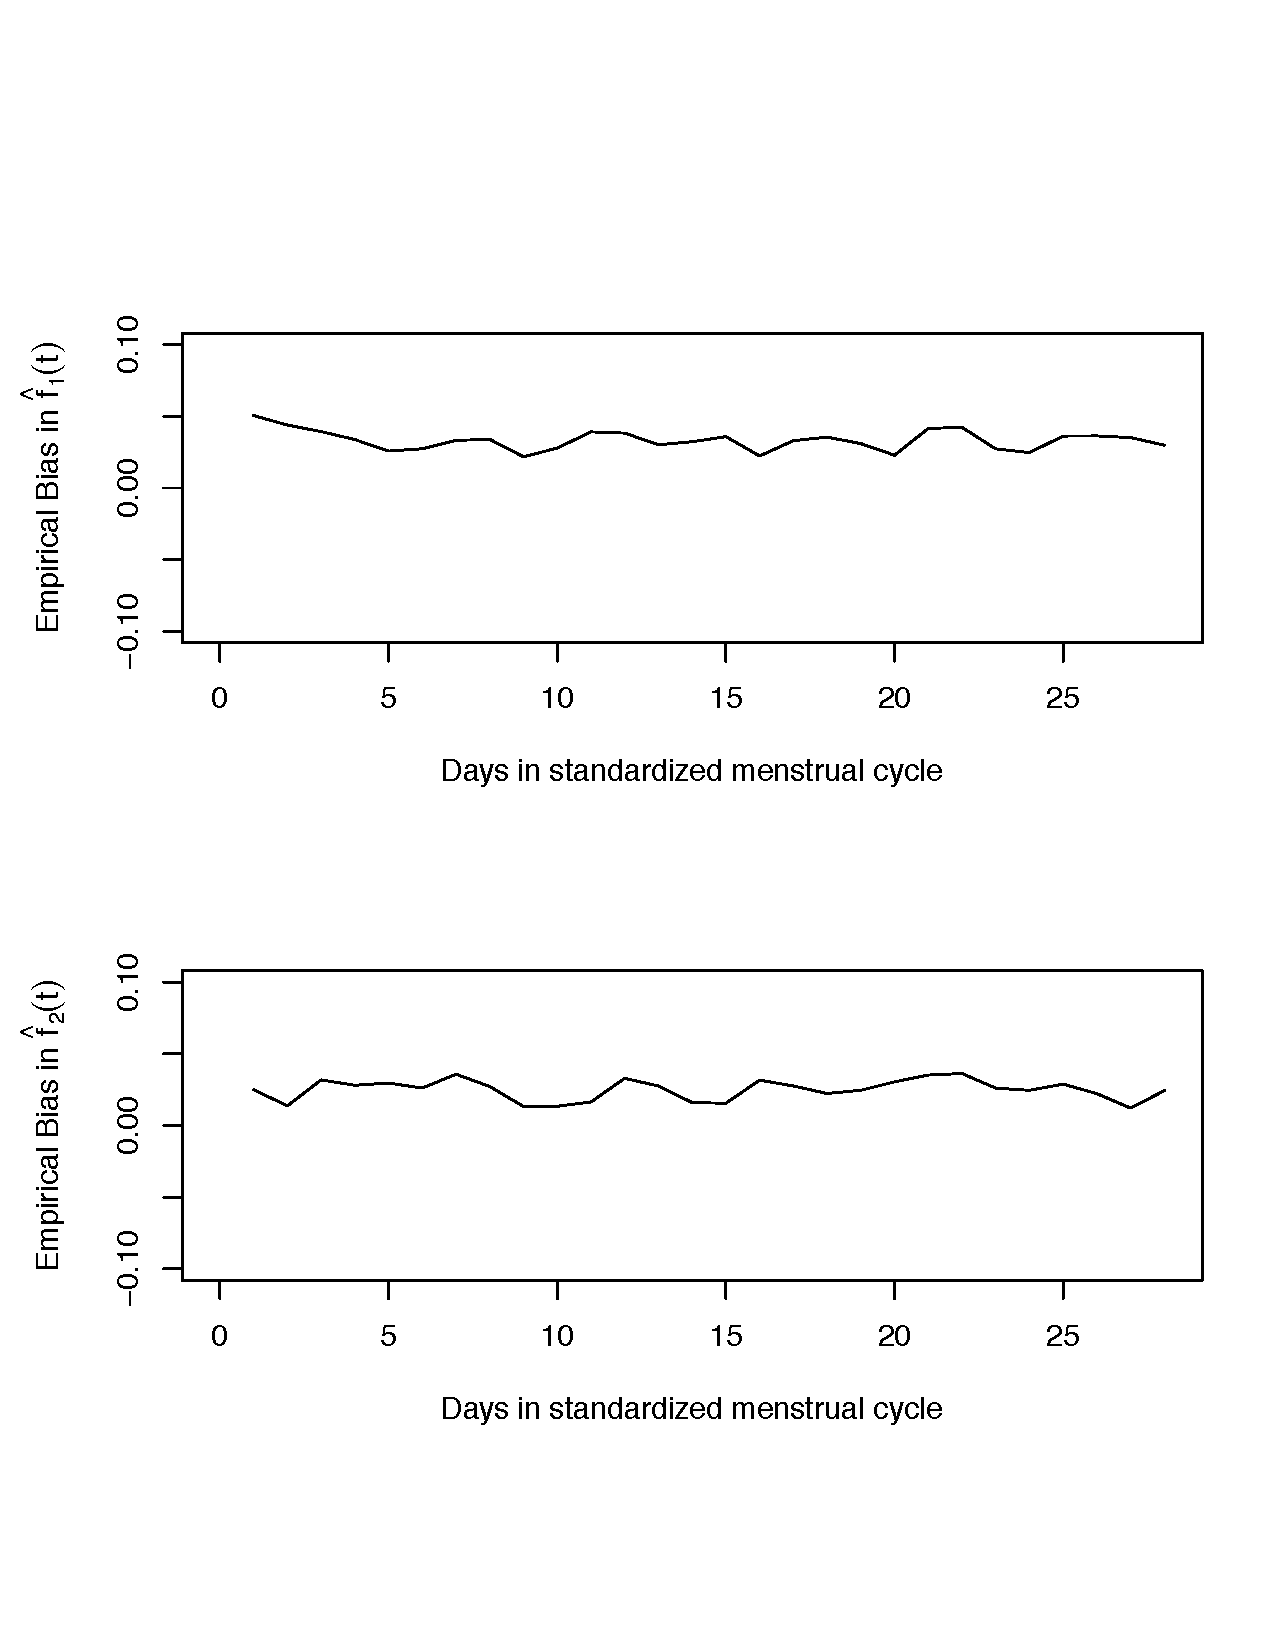
\includegraphics[width=0.7\textwidth]{bivNOU_liu_Biasf.pdf}
% note that files may not be rotated
\caption{Empirical Bias in estimated nonparametric functions $\hat f_1$ and $\hat f_2$ based on 500 simulation replications.}
\label{Biasf}
\end{figure}

\begin{figure}[h!]
\centering
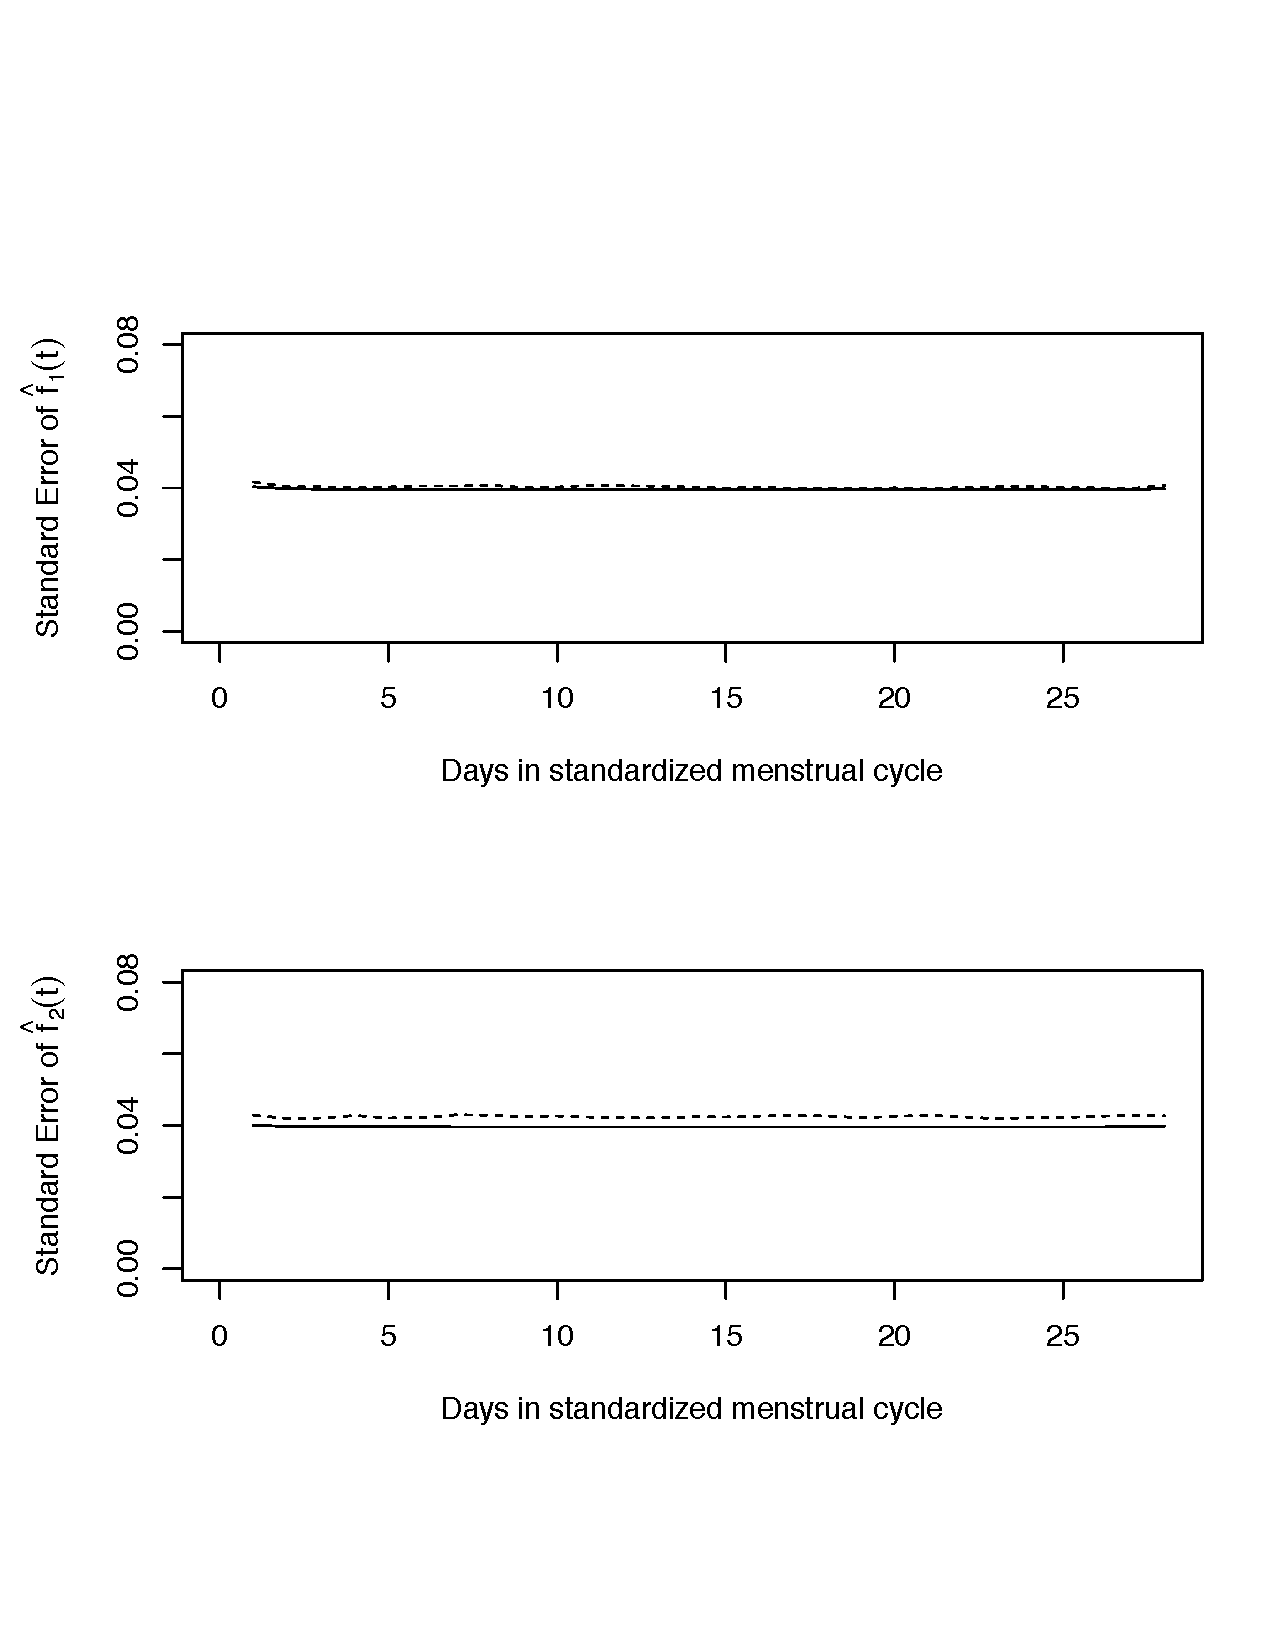
\includegraphics[width=0.7\textwidth]{bivNOU_liu_SEf.pdf}
\caption{Pointwise empirical (dashes) and frequentist (solid) standard errors of the estimated nonparametric functions $\hat f_1$ and $\hat f_2$ based on 500 simulation replications.}
\label{SEf}
\end{figure}

The biases for the nonparametric functions  $\hat f_1$ and $\hat f_2$ are both minimal and center around $0$, see Figure \ref{Biasf}. Figure \ref{SEf} shows that model standard errors of estimates of $\hat f_1$ and $\hat f_2$ agree quite well with the empirical standard errors. 

\begin{figure}[h!]
\centering
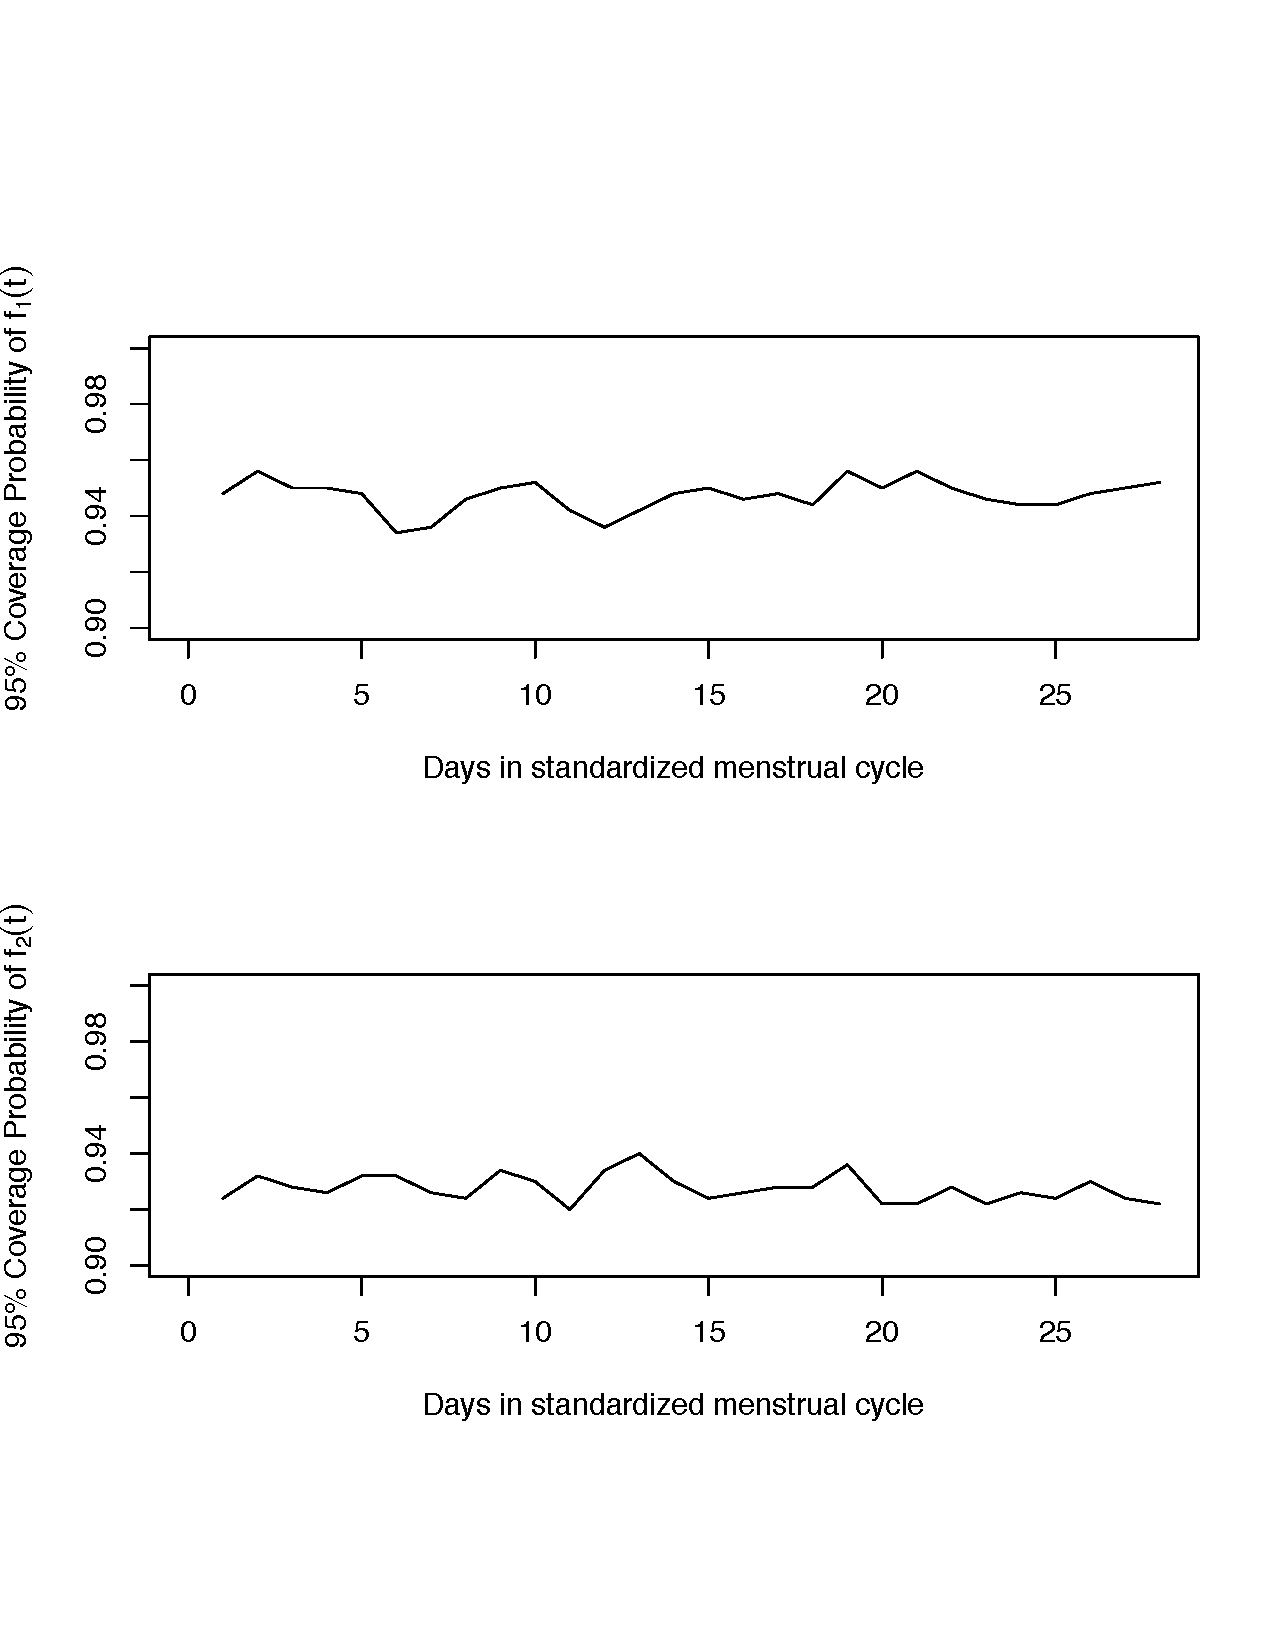
\includegraphics[width=0.7\textwidth]{bivNOU_liu_cp.pdf}
\caption{A graph showing the estimated 95\% coverage probabilities of the true nonparametric functions $f_1$ and $f_2$ based on 500 simulation replications.}
\label{cp}
\end{figure}

Figure \ref{cp} shows the estimated pointwise $95\%$ coverage probabilities of the true nonparametric functions $f_1$ and $f_2$. The means for the estimated coverage probabilities are $95\%$ and $93\%$ for  $\hat f_1$ and $\hat f_2$. Overall, our simulation study results are good.



\subsection{Misspecification of Gaussian Fields}

We further conduct simulation studies when the Gaussian fields are incorrectly specified and study the effect of this misspecification on fixed effects, variance, and smoothing parameter estimations. Specifically, we use OU and Wiener bivariate Gaussian fields, respectively, to analyze datasets generated by NOU bivariate Gaussian field with the same specification as above.

Based on 400 simulations results for each choice of Gaussian field, the estimates of regression coefficients and random intercepts are fairly robust with bias close to zero even when the bivariate Gaussian field is misspecified as bivariate OU or Wiener field. The estimates for the smoothing parameters is much more biased for both bivariate OU or Wiener field, though misspecification in OU field would lead to less bias than that in Wiener. The estimates for variance of the measurement error are almost unbiased with the misspecification of bivariate Wiener field; whereas it is $20\%$ more biased in the case of misspecification of bivariate OU field. In conclusion, misspecification of Gaussian field does not  have a major influence if more emphasis is placed on the estimates of regression coefficients, yet the estimates of smoothing parameters and some variance components can vary significantly from the true values in the presence of misspecification of Gaussian field. 

%======================================================================
%
% DATA ANALYSIS
%
%
%======================================================================

\section{Bivariate Longitudinal Hormone Data Analysis} \label{dataAnalysis}

The model we proposed was motivated by a bivariate longitudinal hormone dataset on progesterone and estrogen.
Daily urine samples were collected from 403 employed women aged $20$ to $44$ years who completed a median of five consecutive menstrual cycles of collection each \cite{Gold:Eske:Lasl:Samu:O'Nei:Over:Sche:quan:1995}. Of these, $338$ women collected daily urine samples for at least one complete menstrual cycle, had fewer than three days of missing data in any five-day rolling window, did not have a conception in the analyzed cycles, and had complete covariate information. One menstrual cycle was randomly selected from each of the $338$ women. 
%Of these, $273$ cycles were determined to be ovulatory cycles using the algorithm of Waller et al. (9) and were included in all of the present analyses. Of these $273$ cycles, 121 had an ovulatory immediately prior cycle and were included in an analysis to investigate the influence of previous cycles on subsequent cycles. 
Risk factor data were obtained by in-person interview at baseline. The details of the study design and assay methods are described in detail previously \cite{Gold:Eske:Lasl:Samu:O'Nei:Over:Sche:quan:1995} and \cite{Gold:Eske:Hamm:Lasl:Samu:O'Nei:Hine:Over:Sche:quan:1995}. 

For demonstration purposes, we randomly select  $100$ study participants from the study, with a total of $5498$ observations for both responses. 
Each woman contributes from $16$ to $43$ observations over a menstrual cycle, resulting an average of $28$ observations per woman.
In order for the results to be biologically meaningful, the menstrual cycle length for each women has been standardized to a reference of $28$ days, based on the assumption that the change of hormone level for each woman depends on the time of the menstrual cycle relative to the cycle length. The standardization generates $56$ distinct time points with increments between time points of 1/2 day each. To make the normality assumption more appropriate, a log transformation was used for each of the two hormones. 

Figure \ref{Liu1} plots the log-transformed progesterone and estrogen levels during a standardized menstrual cycle. Figure \ref{Liu2} plots their empirical sample variances calculated at each distinct time point. 

\begin{figure}[h!]
\centering
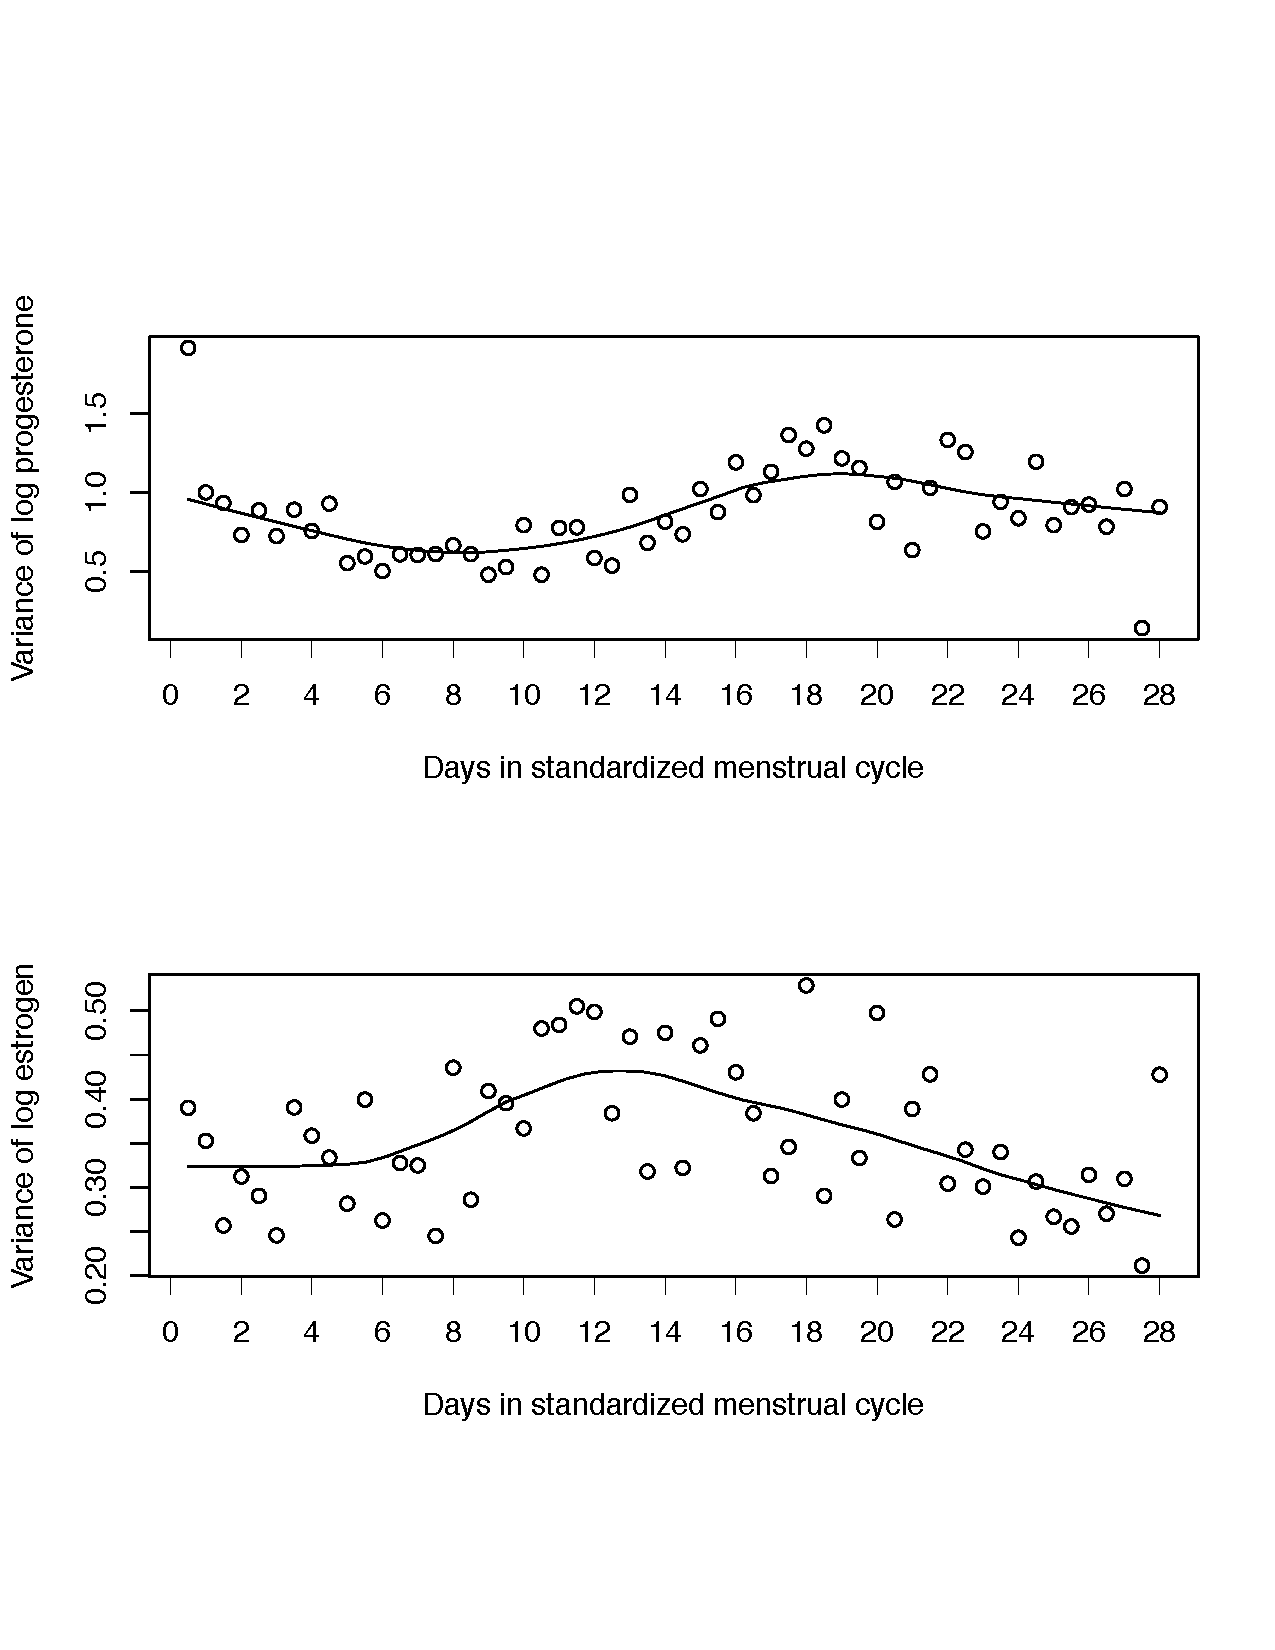
\includegraphics[width=0.7\textwidth]{bivLiuFig2.pdf}
\caption{Plots of empirical sample variance of log progesterone  and log estrogen levels at each distinct time points in a standardized menstrual cycle.}
\label{Liu2}
\end{figure}

Denoting $\{(Y_{1ij}, Y_{2ij})\}$ the $j^{th}$ log-transformed progesterone and estrogen values measured at standardized day $t_{ij}$ since menstruation for the $i^{th}$ woman, we consider the following bivariate semiparametric stochastic mixed model:
\begin{eqnarray*}
Y_{1ij} &=& {\rm age}_i^T  \beta_{11}  + {\rm underWeight}_i^T  \beta_{12}
+ {\rm overWeight}_i^T  \beta_{13}
+ f_1(t_{ij}) + b_{1i} + U_{1i}(t_{ij}) + \epsilon_{1ij} 
 \\
Y_{2ij} &=& {\rm age}_i^T  \beta_{21} +  {\rm underWeight}_i^T  \beta_{22}
+  {\rm overWeight}_i^T  \beta_{23}
+ f_2(t_{ij}) + b_{2i} + U_{2i}(t_{ij}) + \epsilon_{2ij} 
\\
&& i = 1, \dots, 100; j  = 1, \dots, n_i; t_{ij} \in \{0.5, 1.0, \dots, 28\}
\end{eqnarray*}
where the specifications of random intercepts $b_{1i}$ and $b_{2i}$, the bivariate Gaussian field  $U_{1i}$ and $U_{2i}$, the measurement errors $ \epsilon_{1ij} $ and $ \epsilon_{2ij}$, and the nonparametric smooth functions are the same as those in the simulation study. Covariates underWeight and overWeight are indicator variables, which is characterized by Body Mass Index (BMI)  where if BMI is less than 19.0 then the person is categorized as underWeight whereas if BMI is greater than 25.7, then overWeight. 
For computational stability, standardized days were centered at the median day 14 and divided by 10; covariate age is also centered at median 33 years old and divided by 100. Thus, $f_1(t)$ and $f_2(t)$ represents the progesterone and estrogen curves, respectively, for women of 33 years old with normal weight. 

\begin{table}[h!]
\centering
\caption{Estimates of regression coefficients, variance parameter and smoothing parameter for the progesterone and estrogen data.} 
\begin{tabular}{l*{6}{c}r}
\hline
\hline
 Model parameters              & Parameter estimate  & Standard Error  
\\
$\beta_{11}$       & -1.2651         & 1.8674          \\
$\beta_{12}$       & -0.1687         & 0.2995          \\
$\beta_{13}$       & -0.1837         & 0.2009          \\
$\beta_{21}$        & -0.1455         & 1.7131          \\
$\beta_{22}$        &  0.0068         & 0.2747          \\
$\beta_{23}$        &  0.0765         & 0.1843          \\
$\tau_1$   &   4.6081      \\
$\tau_2$   &   1.8475      \\
$\phi_1$   &   0.6455      \\
$\phi_{1,2}$   &  -0.2755      \\
$\phi_2$   &   0.6208      \\
$\sigma_1^2$   &   0.6499      \\
$\sigma_2^2$   &   0.6019      \\
$\rho_1$   &   0.2368      \\
$a_{10}$   &  -0.7699      \\
$a_{11}$   &   0.2894      \\
$a_{12}$   &  -0.1673      \\
$\rho_2$   &   0.0917      \\
$a_{20}$   &  -1.7431      \\
$a_{21}$   &   0.5172      \\
$a_{22}$   &  -0.0800      \\
\hline
\end{tabular}
\label{tableLiu}
\end{table}


Table \ref{tableLiu} records the results of estimates of regression coefficients, smoothing parameters and variance components. The standard errors of our fixed effects parameter estimates are sufficiently large such that none of the fixed effects parameter estimates are statistically significant. That said, in terms of point estimates, we find a negative association on both responses with age, and  both overweight and underweight (compared to regular BMI) are also negatively associated with  progesterone only. 
%The correlation of the random effects,  can be calculated from  
%, ${\rm var}(b_{1}) = \phi_1 = 0.6455$ and ${\rm var}(b_{2}) = \phi_3 =  0.6208$ from the table and it is $-0.4352$, 
The estimated correlation of the bivariate responses can be calculated from variance estimates from Table  \ref{tableLiu}:
\begin{eqnarray*}
&&
{\rm corr}(Y_{1ij}, Y_{2ik}) = {{\rm cov}(Y_{1ij}, Y_{2ik}) \over \sqrt {{\rm var}(Y_{1ij})} \sqrt {{\rm var}(Y_{2ik})}} \\
&=& {\phi_{1,2} \over 
\sqrt {\sigma_1^2 + \phi_1 + \rho_1^0 {\rm exp}\{a_{10} + a_{11}t_{ij} + a_{12}t_{ij}^2 \}} 
\sqrt {\sigma_2^2 + \phi_2 + \rho_2^0 {\rm exp}\{a_{20} + a_{21}t_{ik} + a_{22}t_{ik}^2 \}} } \\
&=& { -0.2755  \over 
\sqrt {0.6499 + 0.6455 + {\rm exp}\{-0.7699 + 0.2894 t_{ij} -0.1673 t_{ij}^2 \}} 
\sqrt {0.6019 + 0.6208 + {\rm exp}\{-1.7431 + 0.5172 t_{ik} -0.0800 t_{ik}^2 \}} },
\end{eqnarray*}
since ${\rm cov}(Y_{1ij}, Y_{2ij}) = {\rm cov}(b_{1}, b_{2})$ in this case.
For example, if $t_{ij} = 5$ and $t_{ik} = 6$, then ${\rm corr}(Y_{1ij}, Y_{2ik}) = -0.2343$, 
which indicates that that the two hormones are negatively correlated when progesterone is at $t_{ij} = 5$ and estrogen is at $t_{ik} = 6$.
% as shown in Figure  \ref{Liu1}.
The estimates of nonparametric function $\hat f_1$ and $\hat f_2$ and their 95\% confidence interval are superimposed over the log responses in Figure  \ref{Liu1}, respectively, which accurately captures the underlying trends of the bivariate longitudinal responses.


%======================================================================
%
% CONCLUSION AND DISCUSSIONS
%
%
%======================================================================
\section{Discussion} \label{discu}

We propose and build a model for analysis of bivariate cyclic longitudinal data and provide inference procedures. The model is proposed in the likelihood framework and the regression parameters and nonparametric functions are estimated by maximizing a penalized likelihood function.  
The smoothing parameter and variance components are numerically estimated using the Fisher-scoring algorithm based on restricted maximum likelihood.
Modelling the time effect nonparametrically gives more flexibility in specifying the response mean structure, and the Gaussian field allows for additional flexibility in specifying the within-subject correlation structure, including possibly non-stationarity. 
The correlation of the two responses were explained only through the correlation of the random effects in the data analysis in Section \ref{dataAnalysis}, though the proposed model \ref{biv} can accommodate more complicated correlation structure of the responses through the covariance matrix (\ref{gfcov}) of the bivariate Gaussian field, as illustrated in subsection \ref{bivRes}. Simulation results show that inference procedure performs well in all estimation results.


The bivariate semiparametric stochastic longitudinal model we proposed can be readily extended to multivariate longitudinal data.   
Dimensionality can pose as a challenge during the extension however. In the bivariate studies, we employed both C++ and parallel computing in the simulation study. Despite the effort, there is still computational burden to this methodology's estimation. Also, special attention was given to parameter initialization as some initialization of parameters may lead to infinity in some entries of variance-covariance matrix, thus causing the matrix degenerate. This said, in the analysis of the real dataset, we tried three very different initializations of the parameters from one another, and all estimates of the regression parameters, the variance components, and smoothing parameters are qualitatively the same, which is reassuring. 


We would like to further explore sensitivity/robustness to the model assumptions. We have investigated the impact of Gaussian field misspecification in the simulation studies, which show that the choice of Gaussian field has little impact on the fixed effect parameters of interest. However, if we were interested in the underlying biological process, a deeper understanding of the choice of the Gaussian field is needed. 
Also, non-Guassian models can be generalized under the proposed framework if needed.
In spite of further work to consider, this is a flexible and informative method for modeling bivariate  longitudinal response data and we look forward to further extensions of this work in the above and possibly other directions.


%=========================================================================
%
% APPENDIX
%
%=========================================================================
\appendix 

\section{}\label{app1}
%------------------------------------------------------------------------------------------------------------------------------
%
% Normal Matrix
%
%
%------------------------------------------------------------------------------------------------------------------------------
\begin{proof}[Proof of (\ref{normalMatrix})]
Taking derivative of the log-likelihood function (\ref{penLog}) with respect to $\bm \beta$, $\bm f_1$, and $\bm f_1$, we have
\begin{eqnarray*}
% Derivatives wrt beta
\ell_{\bm \beta} &=&\boldsymbol X^T  \boldsymbol W
(\boldsymbol Y - \boldsymbol X \boldsymbol \beta 
- \boldsymbol N_1 \boldsymbol f_1 -
\boldsymbol N_2 \boldsymbol f_2) \\
% Derivatives wrt f1 
\ell_{\bm f_1}
&=&
\boldsymbol N_1^T  \boldsymbol W
(\boldsymbol Y - \boldsymbol X \boldsymbol \beta - \boldsymbol N_1 \boldsymbol f_1 -
\boldsymbol N_2 \boldsymbol f_2)
- \lambda_1 \bm K \bm f_1 \\
% Derivatives w.r.t. f2
\ell_{\boldsymbol f_2} 
&=& 
\boldsymbol N_2^T  \boldsymbol W
(\boldsymbol Y - \boldsymbol X \boldsymbol \beta - \boldsymbol N_1 \boldsymbol f_1 -
\boldsymbol N_2 \boldsymbol f_2)
- \lambda_2 \boldsymbol K  \boldsymbol f_2.
\end{eqnarray*}
Set $\ell_{\bm \beta}, \ell_{\bm f_1}$ and $\ell_{\bm f_2}$ to be zero, we have 
\begin{eqnarray}
% NORMAL EQUATION beta
\boldsymbol X^T  \boldsymbol W
(\boldsymbol X \boldsymbol {\hat \beta} 
+  \boldsymbol N_1 \boldsymbol {\hat f}_1
+  \boldsymbol N_2 \boldsymbol {\hat f}_2)
&=&  \boldsymbol X^T  \boldsymbol W \boldsymbol Y 
\label{normal_beta} \\
% NORMAL EQUATION f_1
\boldsymbol N_1^T  \boldsymbol W
(\boldsymbol X \boldsymbol {\hat \beta} +  \boldsymbol N_1 \boldsymbol {\hat f}_1 
+ \boldsymbol N_2 \boldsymbol {\hat f}_2) 
+ \lambda_1 \boldsymbol K \boldsymbol {\hat f_1}
&=&
\boldsymbol N_1^T  \boldsymbol W \boldsymbol Y  
\label{normal_f1} \\
% NORMAL EQUATION f_2
\boldsymbol N_2^T  \boldsymbol W
(\boldsymbol X \boldsymbol {\hat \beta} +  \boldsymbol N_1 \boldsymbol {\hat f}_1 
+ \boldsymbol N_2 \boldsymbol {\hat f}_2) 
+
\lambda_2 \boldsymbol K\boldsymbol {\hat f}_2
&=&  
\boldsymbol N_2^T  \boldsymbol W \boldsymbol Y,
 \label{normal_f2} 
\end{eqnarray}
which can be rewritten as (\ref{normalMatrix}).
\end{proof}
%\begin{proof}[of (\ref{normalMatrix})]
%------------------------------------------------------------------------------------------------------------------------------
%% Derivatives w.r.t. beta
%Taking derivative of the log-likelihood function (\ref{penLog}) with respect to $\boldsymbol \beta$, we have
%\begin{eqnarray*}
%\ell_{\boldsymbol \beta} &=& \left(- {1 \over 2}\right) (-2)  \boldsymbol X^T  \boldsymbol V ^{-1}  
% (\boldsymbol Y - \boldsymbol X \boldsymbol \beta - 
% \boldsymbol N_1 \boldsymbol f_1 -
%  \boldsymbol N_2 \boldsymbol f_2) \\ 
%%&=&\boldsymbol X^T  \boldsymbol W
%% (\boldsymbol Y - \boldsymbol X \boldsymbol \beta 
%% - \boldsymbol N_1 \boldsymbol f_1 -
%%  \boldsymbol N_2 \boldsymbol f_2) \\
% &=&
% \boldsymbol X^T  \boldsymbol W \boldsymbol Y 
% - \boldsymbol X^T  \boldsymbol W\boldsymbol X \boldsymbol \beta 
% - \boldsymbol X^T  \boldsymbol W \boldsymbol N_1 \boldsymbol f_1
%  - \boldsymbol X^T  \boldsymbol W \boldsymbol N_2 \boldsymbol f_2,
%\end{eqnarray*}
%where $\boldsymbol W = \boldsymbol V^{-1}$.
%Set $\ell_{\boldsymbol \beta} = 0$, we have 
%% normal beta
%\begin{equation} \label{normal_beta}
%\boldsymbol X^T  \boldsymbol W
%(\boldsymbol X \boldsymbol {\hat \beta} 
%+  \boldsymbol N_1 \boldsymbol {\hat f}_1
%+  \boldsymbol N_2 \boldsymbol {\hat f}_2)
%=  \boldsymbol X^T  \boldsymbol W \boldsymbol Y.
%\end{equation}
%Rearranging, we have
%\[
%%\begin{equation} \label{beta_hat}
%% beta
% \boldsymbol {\hat \beta} = 
%(\boldsymbol X^T  \boldsymbol W\boldsymbol X)^{-1}  
%\boldsymbol X^T  \boldsymbol W (\boldsymbol Y
% - \boldsymbol N_1 \boldsymbol {\hat f}_1
%  - \boldsymbol N_2 \boldsymbol {\hat f}_2). 
%%\end{equation}
%\]
%%------------------------------------------------------------------------------------------------------------------------------
%% Derivatives w.r.t. f1 
%Similarly, taking derivative of the log-likelihood function (\ref{penLog}) with respect to $\boldsymbol f_1$, we have 
%\begin{eqnarray*}
%\ell_{\boldsymbol f_1} &=& \left(- {1 \over 2}\right) (-2)  \boldsymbol N_1^T  \boldsymbol W
% (\boldsymbol Y - \boldsymbol X \boldsymbol \beta - \boldsymbol N_1 \boldsymbol f_1 -
%  \boldsymbol N_2 \boldsymbol f_2)
% - {\lambda_1 \over 2} (2) \boldsymbol K  \boldsymbol f_1 \\ 
%&=&
% \boldsymbol N_1^T  \boldsymbol W \boldsymbol Y 
% - \boldsymbol N_1^T  \boldsymbol W \boldsymbol X \boldsymbol \beta 
% - \boldsymbol N_1^T  \boldsymbol W \boldsymbol N_1 \boldsymbol f_1 
%  - \boldsymbol N_1^T  \boldsymbol W \boldsymbol N_2 \boldsymbol f_2
% - \lambda_1 \boldsymbol K \boldsymbol f_1.
% \end{eqnarray*}
%Setting  $\ell_{\boldsymbol f_1} = 0$, we have 
%\begin{eqnarray} \label{normal_f1}
%%\boldsymbol N_1^T  \boldsymbol W\boldsymbol X \boldsymbol {\hat \beta} 
%%+ 
%% (\boldsymbol N_1^T  \boldsymbol W \boldsymbol N_1 \boldsymbol 
%% + \lambda_1 \boldsymbol K) \boldsymbol {\hat f}_1 
%%   + \boldsymbol N_1^T  \boldsymbol W \boldsymbol N_2 \boldsymbol {\hat f}_2
%% &=&
%%   \boldsymbol N_1^T  \boldsymbol W \boldsymbol Y \nonumber 
%%   \\
%   \boldsymbol N_1^T  \boldsymbol W
%   (\boldsymbol X \boldsymbol {\hat \beta} +  \boldsymbol N_1 \boldsymbol {\hat f}_1 
%   + \boldsymbol N_2 \boldsymbol {\hat f}_2) 
%   + \boldsymbol\lambda_1 \boldsymbol K \boldsymbol {\hat f_1}
% &=&
%   \boldsymbol N_1^T  \boldsymbol W \boldsymbol Y  
%\end{eqnarray} 
%which gives 
%\begin{equation} \label{hat_f1}
%% ESTIMATE OF f_1
% \boldsymbol {\hat f}_1 
% =  (\boldsymbol N_1^T  \boldsymbol W \boldsymbol N_1 \boldsymbol 
% + \lambda_1 \boldsymbol K)^{-1}
% \boldsymbol N_1^T  \boldsymbol W
%  ( \boldsymbol Y 
% - \boldsymbol X \boldsymbol {\hat \beta}
% -   \boldsymbol N_2 \boldsymbol {\hat f}_2). 
%\end{equation}
%%------------------------------------------------------------------------------------------------------------------------------
%% Derivatives w.r.t. f2
%Further, taking derivative of the log-likelihood function (\ref{penLog}) with respect to $\boldsymbol f_2$, we have 
%\begin{eqnarray*}
%\ell_{\boldsymbol f_2} 
%&=& 
%\left(- {1 \over 2}\right) (-2)  \boldsymbol N_2^T  \boldsymbol W
% (\boldsymbol Y - \boldsymbol X \boldsymbol \beta - \boldsymbol N_1 \boldsymbol f_1 -
%  \boldsymbol N_2 \boldsymbol f_2)
% - {\lambda_2 \over 2} (2) \boldsymbol K  \boldsymbol f_2 \\ 
% &=&
% \boldsymbol N_2^T  \boldsymbol W
% (\boldsymbol Y - \boldsymbol X \boldsymbol \beta - \boldsymbol N_1 \boldsymbol f_1 -
%  \boldsymbol N_2 \boldsymbol f_2)
%  - \lambda_2 \boldsymbol K  \boldsymbol f_2.
%%&=&
%% \boldsymbol N_2^T  \boldsymbol W \boldsymbol Y 
%% - \boldsymbol N_2^T  \boldsymbol W \boldsymbol X \boldsymbol \beta 
%% - \boldsymbol N_2^T  \boldsymbol W \boldsymbol N_1 \boldsymbol f_1 
%%  - \boldsymbol N_2^T  \boldsymbol W \boldsymbol N_2 \boldsymbol f_2
%% - \lambda_2 \boldsymbol K \boldsymbol f_2.
% \end{eqnarray*}
%Setting  $\ell_{\boldsymbol f_2} = 0$, we have 
%\begin{equation} \label{normal_f2}
%% NORMAL EQUATION f_2
%\boldsymbol N_2^T  \boldsymbol W
% (\boldsymbol X \boldsymbol {\hat \beta} +  \boldsymbol N_1 \boldsymbol {\hat f}_1 
%   + \boldsymbol N_2 \boldsymbol {\hat f}_2) 
%  +
%  \lambda_2 \boldsymbol K\boldsymbol {\hat f}_2
% =  
% \boldsymbol N_2^T  \boldsymbol W \boldsymbol Y. 
%\end{equation}
%which give 
%\begin{equation} \label{hat_f2}
%% ESTIMATE OF f_2
% \boldsymbol {\hat f}_2 
% =  (\boldsymbol N_2^T  \boldsymbol W \boldsymbol N_2 \boldsymbol 
% + \lambda_2 \boldsymbol K)^{-1}
%  \boldsymbol N_2^T  \boldsymbol W (\boldsymbol Y -\boldsymbol X \boldsymbol {\hat \beta}
% -  \boldsymbol N_1 \boldsymbol {\hat f}_1). 
%\end{equation}
%In other words, differentiation of (\ref{penLog}) with respect to  $\boldsymbol \beta$,  $\boldsymbol f_1$ and  $\boldsymbol f_2$ solves 
%\[
% \begin{pmatrix}
%  \boldsymbol X^T  \boldsymbol W \boldsymbol X & \boldsymbol X^T  \boldsymbol W \boldsymbol N_1 & \boldsymbol X^T  \boldsymbol W \boldsymbol N_2 \\
%   \boldsymbol N_1^T  \boldsymbol W\boldsymbol X & \boldsymbol N_1^T  \boldsymbol W \boldsymbol N_1 \boldsymbol 
% + \lambda_1 \boldsymbol K &  \boldsymbol N_1^T  \boldsymbol W \boldsymbol N_2  \\
%  \boldsymbol N_2^T  \boldsymbol W\boldsymbol X &  \boldsymbol N_2^T  \boldsymbol W \boldsymbol N_1 & \boldsymbol N_2^T  \boldsymbol W \boldsymbol N_2 \boldsymbol 
% +
%  \lambda_2 \boldsymbol K \\
% \end{pmatrix}
%  \begin{pmatrix}
%   \boldsymbol \beta \\
% \boldsymbol f_1 \\
% \boldsymbol f_2\\
% \end{pmatrix}
%  =
% \begin{pmatrix}
%   \boldsymbol X^T  \boldsymbol W \boldsymbol Y \\
%   \boldsymbol N_1^T  \boldsymbol W \boldsymbol Y  \\
%  \boldsymbol N_2^T  \boldsymbol W \boldsymbol Y  \\
% \end{pmatrix}.
% \]
%\end{proof}

%=========================================================================
%
% FIND EXPLICIT EXPRESSION FOR beta, f1 AND f2.
%
%=========================================================================
\begin{proof} [Proof of (\ref{betaHat}),  (\ref{f1Hat}) and  (\ref{f2Hat})]
From equations (\ref{normal_beta}), (\ref{normal_f1}) and (\ref{normal_f2}), we can reexpress the parameter estimators
\begin{eqnarray} 
% beta
\boldsymbol {\hat \beta}
&=&
(\boldsymbol X^T  \boldsymbol W\boldsymbol X)^{-1}  
\boldsymbol X^T  \boldsymbol W (\boldsymbol Y
- \boldsymbol N_1 \boldsymbol {\hat f}_1
- \boldsymbol N_2 \boldsymbol {\hat f}_2)
% \label{beta_hat} 
\nonumber
\\
% ESTIMATE OF f_1
\boldsymbol {\hat f}_1 
&=&
(\boldsymbol N_1^T  \boldsymbol W \boldsymbol N_1 \boldsymbol 
+ \lambda_1 \boldsymbol K)^{-1}
\boldsymbol N_1^T  \boldsymbol W
( \boldsymbol Y 
- \boldsymbol X \boldsymbol {\hat \beta}
-   \boldsymbol N_2 \boldsymbol {\hat f}_2) 
\label{hat_f1}\\ 
% ESTIMATE OF f_2
\boldsymbol {\hat f}_2 
&=& (\boldsymbol N_2^T  \boldsymbol W \boldsymbol N_2 \boldsymbol 
+ \lambda_2 \boldsymbol K)^{-1}
\boldsymbol N_2^T  \boldsymbol W (\boldsymbol Y -\boldsymbol X \boldsymbol {\hat \beta}
-  \boldsymbol N_1 \boldsymbol {\hat f}_1).  \label{hat_f2}
\end{eqnarray}
To solve explicitly for $\boldsymbol {\hat \beta}$, $\boldsymbol {\hat f_1}$ and $\boldsymbol {\hat f_2}$, we first plug $ \boldsymbol {\hat f_1}$ (\ref{hat_f1}) into equations (\ref{normal_beta}) and  (\ref{normal_f2}), rearrange and obtain 
\begin{eqnarray*} 
&&
\boldsymbol X^T  \boldsymbol W
\big[
\boldsymbol X \boldsymbol {\hat \beta} 
- 
\boldsymbol N_1 
 (\boldsymbol N_1^T  \boldsymbol W \boldsymbol N_1 \boldsymbol 
 + \lambda_1 \boldsymbol K)^{-1}
 \boldsymbol N_1^T  \boldsymbol W
  (\boldsymbol X \boldsymbol {\hat \beta} + \boldsymbol N_2 \boldsymbol {\hat f}_2)
+  \boldsymbol N_2 \boldsymbol {\hat f}_2
\big] \\
&=&
  \boldsymbol X^T  \boldsymbol W \boldsymbol Y
  - \boldsymbol X^T  \boldsymbol W
  \boldsymbol N_1 
 (\boldsymbol N_1^T  \boldsymbol W \boldsymbol N_1 \boldsymbol 
 + \lambda_1 \boldsymbol K)^{-1}
 \boldsymbol N_1^T  \boldsymbol W \boldsymbol Y;
\end{eqnarray*}
and
\begin{eqnarray*} 
&&
\boldsymbol N_2^T  \boldsymbol W
\big[
\boldsymbol X \boldsymbol {\hat \beta} 
- 
\boldsymbol N_1 
(\boldsymbol N_1^T  \boldsymbol W \boldsymbol N_1 \boldsymbol 
+ \lambda_1 \boldsymbol K)^{-1}
\boldsymbol N_1^T  \boldsymbol W
(\boldsymbol X \boldsymbol {\hat \beta} +  \boldsymbol N_2 \boldsymbol {\hat f}_2)
+  \boldsymbol N_2 \boldsymbol {\hat f}_2
\big] \\
&=&
  \boldsymbol N_2^T  \boldsymbol W
 \boldsymbol Y
  - \boldsymbol N_2^T  \boldsymbol W
  \boldsymbol N_1 
 (\boldsymbol N_1^T  \boldsymbol W \boldsymbol N_1 \boldsymbol 
 + \lambda_1 \boldsymbol K)^{-1}
 \boldsymbol N_1^T  \boldsymbol W \boldsymbol Y
\end{eqnarray*}
respectively; 
which can be rewritten as
\begin{equation} \label{normal_new_beta}
\boldsymbol X^T  \boldsymbol W_1
\boldsymbol X \boldsymbol {\hat \beta} 
+ 
\boldsymbol X^T  \boldsymbol W_1
\boldsymbol N_2 \boldsymbol {\hat f}_2
=
\boldsymbol X^T  \boldsymbol W_1
\boldsymbol Y
\end{equation}
and
\begin{equation} \label{normal_new_f2}
% NORMAL_NEW f_2
\boldsymbol N_2^T  \boldsymbol W_1
\boldsymbol X \boldsymbol {\hat \beta} 
+ 
(\boldsymbol N_2^T  \boldsymbol W_1
\boldsymbol N_2 + \boldsymbol \lambda_2 \boldsymbol K)
\boldsymbol {\hat f}_2
=
\boldsymbol N_2^T  \boldsymbol W_1
\boldsymbol Y
\end{equation}
respectively,
where 
% W_1
$\boldsymbol W_1 =
 \boldsymbol W 
 -
\boldsymbol W \boldsymbol N_1 
 (\boldsymbol N_1^T  \boldsymbol W \boldsymbol N_1 \boldsymbol 
 + \lambda_1 \boldsymbol K)^{-1} 
 \boldsymbol N_1^T  \boldsymbol W$.
Or equivalently as 
\begin{equation} \label{beta_hat}
% ESTIMATE of beta
\boldsymbol {\hat \beta} 
= 
(\boldsymbol X^T  \boldsymbol W_1\boldsymbol X)^{-1}  
\boldsymbol X^T  \boldsymbol W_1 (\boldsymbol Y
- \boldsymbol N_2 \boldsymbol {\hat f}_2), 
\end{equation}
and
\begin{equation}   \label{f_2}
% ESTIMATE of f_2
\boldsymbol {\hat f}_2 
=  (\boldsymbol N_2^T  \boldsymbol W_1 \boldsymbol N_2 \boldsymbol 
+ \lambda_2 \boldsymbol K)^{-1}
\boldsymbol N_2^T  \boldsymbol W_1 (\boldsymbol Y -\boldsymbol X \boldsymbol {\hat \beta})
\end{equation}
respectively.
Then  plugging (\ref{beta_hat}) into  (\ref{normal_new_f2})
and (\ref{f_2}) into (\ref{normal_new_beta}) and rearrange, we have
\begin{eqnarray*}
&&
(\boldsymbol N_2^T  \boldsymbol W_1
\boldsymbol N_2 + \boldsymbol \lambda_2 \boldsymbol K)
\boldsymbol {\hat f}_2
-
\boldsymbol N_2^T  \boldsymbol W_1
\boldsymbol X 
(\boldsymbol X^T  \boldsymbol W_1\boldsymbol X)^{-1}  
\boldsymbol X^T  \boldsymbol W_1
\boldsymbol N_2 \boldsymbol {\hat f}_2 \\
&=&
\boldsymbol N_2^T  \boldsymbol W_1
\boldsymbol Y - \boldsymbol N_2^T  \boldsymbol W_1
\boldsymbol X 
(\boldsymbol X^T  \boldsymbol W_1\boldsymbol X)^{-1}  
\boldsymbol X^T  \boldsymbol W_1
\boldsymbol Y,
\end{eqnarray*}
and
\begin{eqnarray*}
&&
\boldsymbol X^T  \boldsymbol W_1
\boldsymbol X \boldsymbol {\hat \beta} 
- 
\boldsymbol X^T  \boldsymbol W_1
\boldsymbol N_2  
(\boldsymbol N_2^T  \boldsymbol W_1 \boldsymbol N_2 \boldsymbol 
 + \lambda_2 \boldsymbol K)^{-1}
  \boldsymbol N_2^T  \boldsymbol W_1 \boldsymbol X \boldsymbol {\hat \beta} \\
&=& 
\boldsymbol X^T  \boldsymbol W_1
\boldsymbol Y
-
\boldsymbol X^T  \boldsymbol W_1
\boldsymbol N_2  
(\boldsymbol N_2^T  \boldsymbol W_1 \boldsymbol N_2 \boldsymbol 
 + \lambda_2 \boldsymbol K)^{-1}
  \boldsymbol N_2^T  \boldsymbol W_1 \boldsymbol Y,
\end{eqnarray*}
respectively.
Therefore, after rearranging and regrouping terms, the closed-form solutions for $ \boldsymbol {\hat f}_2 $ and $\boldsymbol {\hat \beta}$ are
$$
 \boldsymbol {\hat f}_2 
 =  (\boldsymbol N_2^T  \boldsymbol W_{f_2} \boldsymbol N_2 \boldsymbol 
 + \lambda_2 \boldsymbol K)^{-1}
  \boldsymbol N_2^T  \boldsymbol W_{f_2} \boldsymbol Y,
$$
and
$$
\boldsymbol {\hat \beta} 
 = 
 (\boldsymbol X^T  \boldsymbol W_x \boldsymbol X )^{-1} \boldsymbol X^T  \boldsymbol W_x \boldsymbol Y,
$$
where  
% W_{f_2}
$\boldsymbol W_{f_2}  =  \boldsymbol W_1 - \boldsymbol W_1\boldsymbol X(\boldsymbol X^T  \boldsymbol W_1\boldsymbol X)^{-1}  \boldsymbol X^T  \boldsymbol W_1$,
and
$\boldsymbol W_x =
 \boldsymbol W_1 
 -
\boldsymbol W_1 \boldsymbol N_2 
 (\boldsymbol N_2^T  \boldsymbol W_1 \boldsymbol N_2 \boldsymbol 
 + \lambda_2 \boldsymbol K)^{-1} 
 \boldsymbol N_2^T  \boldsymbol W_1$.
%------------------------------------------------------------------------------------------------------------------------------
Similarly, to obtain the closed-form solution for $\boldsymbol {\hat f_1}$, we plug  (\ref{hat_f2}) into equation (\ref{normal_f1}) and obtain
\begin{equation} \label{normal_new_f1}
%\boldsymbol X^T  \boldsymbol W_2
%\boldsymbol X \boldsymbol {\hat \beta} 
%+ 
%\boldsymbol X^T  \boldsymbol W_2
%\boldsymbol N_1 \boldsymbol {\hat f}_1
%&=&
%\boldsymbol X^T  \boldsymbol W_2
%\boldsymbol Y \nonumber
%\\
\boldsymbol N_1^T  \boldsymbol W_2
\boldsymbol X \boldsymbol {\hat \beta} 
+ 
(\boldsymbol N_1^T  \boldsymbol W_2
\boldsymbol N_1 + \boldsymbol \lambda_1 \boldsymbol K)
\boldsymbol {\hat f}_1
=
\boldsymbol N_1^T  \boldsymbol W_2
\boldsymbol Y,
\end{equation}
where 
% W_2
$\boldsymbol W_2 =
 \boldsymbol W 
 -
\boldsymbol W \boldsymbol N_2 
 (\boldsymbol N_1^T  \boldsymbol W \boldsymbol N_1 \boldsymbol 
 + \lambda_1 \boldsymbol K)^{-1} 
 \boldsymbol N_2^T  \boldsymbol W$.
Plugging $ \boldsymbol {\hat \beta} = 
(\boldsymbol X^T  \boldsymbol W_2\boldsymbol X)^{-1}  
\boldsymbol X^T  \boldsymbol W_2 (\boldsymbol Y
  - \boldsymbol N_1 \boldsymbol {\hat f}_1) 
$
into  (\ref{normal_new_f1}), the closed-form solution for $ \boldsymbol {\hat f}_1$ is
$$
 \boldsymbol {\hat f_1} 
 =
  (\boldsymbol N_1^T 
\boldsymbol W_{f_1}  \boldsymbol N_1
  + \lambda_1 \boldsymbol K)^{-1}  \boldsymbol N_1^T \boldsymbol W_{f_1} \boldsymbol Y,
  $$
 where
 $\boldsymbol W_{f_1}  =  \boldsymbol W_2 - \boldsymbol W_2\boldsymbol X(\boldsymbol X^T  \boldsymbol W_2\boldsymbol X)^{-1}  \boldsymbol X^T  \boldsymbol W_2$.  
 \end{proof}

%=========================================================================
%
% FIND EXPLICIT EXPRESSION FOR beta, f1 AND f2.
%
%=========================================================================

\begin{proof} [Proof of (\ref{bHat}) and  (\ref{uHat})]
% From (\ref{condM}), (\ref{bDis}) and (\ref{uDis}), it follows that 
From model assumptions, it follows that 
$$
\boldsymbol Y \sim
N_{2n} \left(\bm{X}\bm{\beta} + \bm N_{1} \bm f_1 + \bm N_{2} \bm f_2,  \bm V \right), \ 
% DISTRIBUTION OF b
\bm b \sim N_{2m} (\bm 0, \bm D).
$$
Since the covariance of $\bm Y$ and $\bm b$ is
\begin{eqnarray*}
{\rm cov} (\boldsymbol Y, \boldsymbol b) &=& {\rm cov}(\boldsymbol{X}\boldsymbol{\beta} +
\boldsymbol N_1 \boldsymbol f_1 + 
\boldsymbol N_2 \boldsymbol f_2 + 
\boldsymbol{Z}\boldsymbol{b} + 
\boldsymbol U + 
\boldsymbol \epsilon, \boldsymbol b) \\ 
&=& {\rm cov}(\boldsymbol{X}\boldsymbol{\beta}, \boldsymbol b)  +
{\rm cov}( \boldsymbol N_1 \boldsymbol f_1,  \boldsymbol b)+ 
{\rm cov}(\boldsymbol N_2 \boldsymbol f_2, \boldsymbol b) 
%  \\&&  
+ 
\boldsymbol{Z}{\rm cov}(\boldsymbol{b}, \boldsymbol b) + 
{\rm cov}(\boldsymbol U, \boldsymbol b) + 
{\rm cov}(\boldsymbol \epsilon, \boldsymbol b) \\
&=& ZD,
\end{eqnarray*}
%Since ${\rm cov} (\bm Y, \bm b) = \bm Z \bm D$, we have
the joint distribution of $\bm Y$ and $\bm b$ is
 \[
 \begin{pmatrix}
  \boldsymbol Y \\
  \boldsymbol b
 \end{pmatrix}
 \sim 
 \boldsymbol N_{2n + 2m} 
 \left(
 \begin{pmatrix}
 \boldsymbol{X}\boldsymbol{\beta} + \boldsymbol N_{1} \boldsymbol f_1 +  \boldsymbol N_{2} \boldsymbol f_2 \\
\boldsymbol 0
 \end{pmatrix},
  \begin{pmatrix}
  \boldsymbol V &  \boldsymbol Z\boldsymbol D \\
  \boldsymbol D\boldsymbol Z^T & D 
 \end{pmatrix}
 \right).
\]
Therefore, by the property of normality, the conditional expectation results follows.
%$$ 
%E(\boldsymbol b | \boldsymbol Y) = \boldsymbol 0 
%+   \boldsymbol D\boldsymbol Z^T   \boldsymbol V^{-1} 
%(\boldsymbol Y - \boldsymbol{X}\boldsymbol{\hat \beta} -
% \boldsymbol N_1 \boldsymbol {\hat f_1} -
%  \boldsymbol N_2 \boldsymbol {\hat f_2})
%  = \boldsymbol D\boldsymbol Z^T   \boldsymbol V^{-1} 
%(\boldsymbol Y - \boldsymbol{X}\boldsymbol{\hat \beta} -
% \boldsymbol N_1 \boldsymbol {\hat f_1} -
%  \boldsymbol N_2 \boldsymbol {\hat f_2})
%$$
\end{proof}


%=========================================================================
%
% Bias of Beta hat,  f1 hat, and f2 hat
%
%=========================================================================

\section{} \label{app2}
% \label{appBiasCov}

\begin{proof} [Proof of (\ref{biasBeta}) and (\ref{biasF1})]
For regression coefficient estimator $\boldsymbol {\hat \beta}$,
%-------------------------------------------------------------------------------------------------
% E(beta)
\begin{eqnarray*}
{\rm E}(\boldsymbol {\hat \beta}) 
&=& 
(\boldsymbol X^T  \boldsymbol W_x \boldsymbol X )^{-1} \boldsymbol X^T  \boldsymbol W_x 
E [ \boldsymbol Y] \\
&=&
(\boldsymbol X^T  \boldsymbol W_x \boldsymbol X )^{-1} \boldsymbol X^T  \boldsymbol W_x 
(\boldsymbol X \boldsymbol \beta +
 \boldsymbol N_{1} \boldsymbol f_1 + 
  \boldsymbol N_{2} \boldsymbol f_2) \\ 
%&=&
%(\boldsymbol X^T  \boldsymbol W_x \boldsymbol X )^{-1} \boldsymbol X^T  \boldsymbol W_x 
%\boldsymbol X \boldsymbol \beta 
%+ (\boldsymbol X^T  \boldsymbol W_x \boldsymbol X )^{-1} \boldsymbol X^T  \boldsymbol W_x   (\boldsymbol N_{1} \boldsymbol f_1 + 
%  \boldsymbol N_{2} \boldsymbol f_2) \\
&=&
 \boldsymbol \beta 
+ (\boldsymbol X^T  \boldsymbol W_x \boldsymbol X )^{-1} \boldsymbol X^T  \boldsymbol W_x   (\boldsymbol N_{1} \boldsymbol f_1 + 
  \boldsymbol N_{2} \boldsymbol f_2)
\end{eqnarray*}
%Or equivalently, we have 
%% E(hat BETA)
%\begin{equation} \label{biasBeta}
%{\rm E}(\boldsymbol {\hat \beta})  -  \boldsymbol \beta  
%= 
%(\boldsymbol X^T  \boldsymbol W_x \boldsymbol X )^{-1} \boldsymbol X^T  \boldsymbol W_x 
%(\boldsymbol N_{1} \boldsymbol f_1 + 
%  \boldsymbol N_{2} \boldsymbol f_2). 
%\end{equation}
%-------------------------------------------------------------------------------------------------
% hat f1
For nonparametric function estimator 
$
\boldsymbol {\hat f}_1
 =
  (\boldsymbol N_1^T 
\boldsymbol W_{f_1}  \boldsymbol N_1
  + \lambda_1 \boldsymbol K)^{-1}  \boldsymbol N_1^T \boldsymbol W_{f_1} \boldsymbol Y
$,
% E(f1)
\begin{eqnarray*}
    {\rm E}(\boldsymbol {\hat f}_1) 
%&=& 
%(\boldsymbol N_1^T 
%\boldsymbol W_{f_1}  \boldsymbol N_1
%+ \lambda_1 \boldsymbol K)^{-1}  \boldsymbol N_1^T \boldsymbol W_{f_1}
%E [ \boldsymbol Y] \\
&=&
(\boldsymbol N_1^T 
\boldsymbol W_{f_1}  \boldsymbol N_1
  + \lambda_1 \boldsymbol K)^{-1}  \boldsymbol N_1^T \boldsymbol W_{f_1}
(\boldsymbol X \boldsymbol \beta + \boldsymbol N_{1} \boldsymbol f_1 + 
  \boldsymbol N_{2} \boldsymbol f_2) \\ 
%&=&
%(\boldsymbol N_1^T \boldsymbol W_{f_1}  \boldsymbol N_1 + \lambda_1 \boldsymbol K)^{-1}  \boldsymbol N_1^T \boldsymbol W_{f_1}
%\boldsymbol X \boldsymbol \beta 
%+ 
%(\boldsymbol N_1^T 
%\boldsymbol W_{f_1}  \boldsymbol N_1 + \lambda_1 \boldsymbol K)^{-1}  
%\boldsymbol N_1^T \boldsymbol W_{f_1}
%\boldsymbol N_{1} \boldsymbol f_1
%\\
%&&\quad\quad\quad\quad\quad
%+
%(\boldsymbol N_1^T \boldsymbol W_{f_1}  \boldsymbol N_1 +  \lambda_1 \boldsymbol K)^{-1}  
%\boldsymbol N_1^T \boldsymbol W_{f_1}
%\boldsymbol N_{2} \boldsymbol f_2\\
   &=&
\boldsymbol 0 
 + (\boldsymbol N_1^T \boldsymbol W_{f_1}  \boldsymbol N_1 + \lambda_1 \boldsymbol K)^{-1}  
(\boldsymbol N_1^T \boldsymbol W_{f_1} \boldsymbol N_{1}+ \lambda_1 \boldsymbol K
 - \lambda_1 \boldsymbol K)
  \boldsymbol f_1\\
&&\quad\quad\quad\quad\quad
+ 
(\boldsymbol N_1^T \boldsymbol W_{f_1}  \boldsymbol N_1
+ 
 \lambda_1 \boldsymbol K)^{-1}  \boldsymbol N_1^T \boldsymbol W_{f_1}
\boldsymbol N_{2} \boldsymbol f_2\\
     &=&
\boldsymbol f_1 
- \lambda_1 
(\boldsymbol N_1^T \boldsymbol W_{f_1}  \boldsymbol N_1 +  \lambda_1 \boldsymbol K)^{-1}   \boldsymbol K \boldsymbol f_1
+ 
(\boldsymbol N_1^T \boldsymbol W_{f_1}  \boldsymbol N_1 +  \lambda_1 \boldsymbol K)^{-1}  \boldsymbol N_1^T \boldsymbol W_{f_1}
\boldsymbol N_{2} \boldsymbol f_2 
%\\
%&=&
%  \boldsymbol f_1 +
%(\boldsymbol N_1^T \boldsymbol W_{f_1}  \boldsymbol N_1 + \lambda_1 \boldsymbol K)^{-1}  
%  ( \boldsymbol N_1^T \boldsymbol W_{f_1}
%  \boldsymbol N_2 \boldsymbol f_2 - \lambda_1    \boldsymbol K \boldsymbol f_1)
\end{eqnarray*}
% SHOW FIRST TERM = 0
where
$(\boldsymbol N_1^T \boldsymbol W_{f_1}  \boldsymbol N_1
  + \lambda_1 \boldsymbol K)^{-1}  \boldsymbol N_1^T \boldsymbol W_{f_1}
  \boldsymbol X \boldsymbol \beta =  \boldsymbol 0$ 
since 
\begin{eqnarray*}
&&(\boldsymbol N_1^T \boldsymbol W_{f_1}  \boldsymbol N_1
  + \lambda_1 \boldsymbol K)^{-1}  \boldsymbol N_1^T \boldsymbol W_{f_1}
  \boldsymbol X \boldsymbol \beta \\
  % PLUG IN W_f1
  &=&
(\boldsymbol N_1^T \boldsymbol W_{f_1}  \boldsymbol N_1
  + \lambda_1 \boldsymbol K)^{-1}  \boldsymbol N_1^T
  \left[
\boldsymbol W_2 - \boldsymbol W_2\boldsymbol X(\boldsymbol X^T  \boldsymbol W_2\boldsymbol X)^{-1}  \boldsymbol X^T  \boldsymbol W_2
  \right]
  \boldsymbol X \boldsymbol \beta 
  \\
  &=&
(\boldsymbol N_1^T \boldsymbol W_{f_1}  \boldsymbol N_1
  + \lambda_1 \boldsymbol K)^{-1}  \boldsymbol N_1^T
\boldsymbol W_2
\boldsymbol X \boldsymbol \beta 
%&&\quad\quad\quad\quad\quad
 -   (\boldsymbol N_1^T \boldsymbol W_{f_1}  \boldsymbol N_1
  + \lambda_1 \boldsymbol K)^{-1}  \boldsymbol N_1^T
\boldsymbol W_2 \boldsymbol X
(\boldsymbol X^T  \boldsymbol W_2\boldsymbol X)^{-1}  
\boldsymbol X^T  \boldsymbol W_2 \boldsymbol X
\boldsymbol \beta  \\
%   &=&
%  (\boldsymbol N_1^T \boldsymbol W_{f_1}  \boldsymbol N_1
%  + \lambda_1 \boldsymbol K)^{-1}  \boldsymbol N_1^T
%\boldsymbol W_2
%\boldsymbol X \boldsymbol \beta 
% -  
%(\boldsymbol N_1^T \boldsymbol W_{f_1}  \boldsymbol N_1 + \lambda_1 \boldsymbol K)^{-1}  \boldsymbol N_1^T
%\boldsymbol W_2
%\boldsymbol X \boldsymbol \beta   \\
  &=&   \boldsymbol 0.
\end{eqnarray*}
%Thus, the bias of $\bm {\hat f_1}$ is 
%% FINAL RESULT E(F1) - F1
%$$
%{\rm E}(\boldsymbol {\hat f_1}) - \boldsymbol { f_1}
%=
%(\boldsymbol N_1^T \boldsymbol W_{f_1}  \boldsymbol N_1 
%+ \lambda_1 \boldsymbol K)^{-1}  
%  ( \boldsymbol N_1^T \boldsymbol W_{f_1}
%  \boldsymbol N_2 \boldsymbol f_2 - \lambda_1    \boldsymbol K \boldsymbol f_1)
%$$
\end{proof}
\begin{rmk}
The bias of nonparametric function estimator $\bm {\hat f}_2$ in (\ref{biasF2}) can be derived similarly as that of $\bm {\hat f}_1$.
\end{rmk}


%------------------------------------------------------------------------------------------------------------------------------
%
% Bias converges to 0
%
%------------------------------------------------------------------------------------------------------------------------------
\begin{lem} \label{biasConv}
The biases of $\boldsymbol {\hat \beta}$, $\boldsymbol {\hat f}_1$, $\boldsymbol {\hat f}_2$, $\boldsymbol {\hat b}_i$ and $\boldsymbol {\hat U}_i$ all go to $\boldsymbol 0$ as both smoothing parameters $\lambda_1 \to 0$ and $\lambda_2 \to 0$.
\end{lem}

\begin{proof}
%-------------------------------------------------------------------------------------------------
% \lambda -> 0
As $\lambda_1 \to 0$ and $\lambda_2 \to 0$ simultaneously, then  
\begin{equation} \label{WxAsy}
\boldsymbol W_x  \to  \boldsymbol W_1 
-
\boldsymbol W_1 \boldsymbol N_2 
(\boldsymbol N_2^T  \boldsymbol W_1 \boldsymbol N_2 \boldsymbol )^{-1} 
\boldsymbol N_2^T  \boldsymbol W_1,
\end{equation}
where 
\begin{equation} \label{W1Asy}
 \boldsymbol W_1 \to
\boldsymbol W 
-
\boldsymbol W \boldsymbol N_1 
(\boldsymbol N_1^T  \boldsymbol W \boldsymbol N_1 \boldsymbol)^{-1} 
\boldsymbol N_1^T  \boldsymbol W
\end{equation}
Plugging $\bm W_x$ in (\ref{WxAsy}) into bias of $\bm {\hat \beta}$ in (\ref{biasBeta}), we have 
\begin{eqnarray}
&& 
{\rm E}(\boldsymbol {\hat \beta})  -  \boldsymbol \beta  \nonumber \\
% STEP 1
&=& 
(\boldsymbol X^T  \boldsymbol W_x \boldsymbol X )^{-1} \boldsymbol X^T 
\left[\boldsymbol W_1 
-
\boldsymbol W_1 \boldsymbol N_2 
(\boldsymbol N_2^T  \boldsymbol W_1 \boldsymbol N_2 \boldsymbol )^{-1} 
\boldsymbol N_2^T  \boldsymbol W_1 \right] 
(\boldsymbol N_{1} \boldsymbol f_1 + 
\boldsymbol N_{2} \boldsymbol f_2) \nonumber\\
% STEP 2
&=& 
(\boldsymbol X^T  \boldsymbol W_x \boldsymbol X )^{-1} \boldsymbol X^T 
\boldsymbol W_1 (\boldsymbol N_{1} \boldsymbol f_1 + 
\boldsymbol N_{2} \boldsymbol f_2) \nonumber\\
&& \hspace{4cm}
-
(\boldsymbol X^T  \boldsymbol W_x \boldsymbol X )^{-1} \boldsymbol X^T
\boldsymbol W_1 \boldsymbol N_2 
(\boldsymbol N_2^T  \boldsymbol W_1 \boldsymbol N_2 \boldsymbol )^{-1} 
\boldsymbol N_2^T  \boldsymbol W_1 
(\boldsymbol N_{1} \boldsymbol f_1 + 
\boldsymbol N_{2} \boldsymbol f_2) \nonumber\\
% STEP 3
&=& 
(\boldsymbol X^T  \boldsymbol W_x \boldsymbol X )^{-1} \boldsymbol X^T 
\boldsymbol W_1 \boldsymbol N_{1} \boldsymbol f_1 \nonumber\\
&& 
+ 
(\boldsymbol X^T  \boldsymbol W_x \boldsymbol X )^{-1} \boldsymbol X^T 
\boldsymbol W_1 \boldsymbol N_{2} 
\left[\boldsymbol f_2 - (\boldsymbol N_2^T  \boldsymbol W_1 \boldsymbol N_2 \boldsymbol )^{-1} 
\boldsymbol N_2^T  \boldsymbol W_1 
\boldsymbol N_{2} \boldsymbol f_2 \right] \nonumber\\ 
&& 
-
(\boldsymbol X^T  \boldsymbol W_x \boldsymbol X )^{-1} \boldsymbol X^T
\boldsymbol W_1 \boldsymbol N_2 
(\boldsymbol N_2^T  \boldsymbol W_1 \boldsymbol N_2 \boldsymbol )^{-1} 
\boldsymbol N_2^T  \boldsymbol W_1 
\boldsymbol N_{1} \boldsymbol f_1 \nonumber\\
% STEP 4
%&=&  \label{rednbiasBeta}
%(\boldsymbol X^T  \boldsymbol W_x \boldsymbol X )^{-1} \boldsymbol X^T 
%\left[\boldsymbol W_1 
%-
%\boldsymbol W_1 \boldsymbol N_2 
%(\boldsymbol N_2^T  \boldsymbol W_1 \boldsymbol N_2 \boldsymbol )^{-1} 
%\boldsymbol N_2^T  \boldsymbol W_1 \right]
%\boldsymbol N_{1} \boldsymbol f_1 \nonumber \\
&=&  \label{rednbiasBeta}
(\boldsymbol X^T  \boldsymbol W_x \boldsymbol X )^{-1} \boldsymbol X^T 
\boldsymbol W_1 \boldsymbol N_{1} \boldsymbol f_1 
-
(\boldsymbol X^T  \boldsymbol W_x \boldsymbol X )^{-1} \boldsymbol X^T 
\boldsymbol W_1 \boldsymbol N_2 
(\boldsymbol N_2^T  \boldsymbol W_1 \boldsymbol N_2 \boldsymbol )^{-1} 
\boldsymbol N_2^T \boldsymbol W_1
\boldsymbol N_{1} \boldsymbol f_1 
%% STEP 5
%&=& \label{rednbiasBeta}
%(\boldsymbol X^T  \boldsymbol W_x \boldsymbol X )^{-1} \boldsymbol X^T 
%\boldsymbol W_x 
%\boldsymbol N_{1} \boldsymbol f_1 
\end{eqnarray}
Further, plugging  $\bm W_1$ in (\ref{W1Asy}) into(\ref{rednbiasBeta}), we have 
\begin{eqnarray*}
&& 
{\rm E}(\boldsymbol {\hat \beta})  -  \boldsymbol \beta  \nonumber \\
%% STEP 1
%&=& 
%(\boldsymbol X^T  \boldsymbol W_x \boldsymbol X )^{-1} \boldsymbol X^T 
%\boldsymbol W_1 \boldsymbol N_{1} \boldsymbol f_1 
%-
%(\boldsymbol X^T  \boldsymbol W_x \boldsymbol X )^{-1} \boldsymbol X^T 
%\boldsymbol W_1 \boldsymbol N_2 
%(\boldsymbol N_2^T  \boldsymbol W_1 \boldsymbol N_2 \boldsymbol )^{-1} 
%\boldsymbol N_2^T \boldsymbol W_1
%\boldsymbol N_{1} \boldsymbol f_1  \\
% STEP 2
&=& 
(\boldsymbol X^T  \boldsymbol W_x \boldsymbol X )^{-1} \boldsymbol X^T 
\left[\boldsymbol W 
-
\boldsymbol W \boldsymbol N_1 
(\boldsymbol N_1^T  \boldsymbol W \boldsymbol N_1 \boldsymbol)^{-1} 
\boldsymbol N_1^T  \boldsymbol W \right] \boldsymbol N_{1} \boldsymbol f_1 \\
&&
-
(\boldsymbol X^T  \boldsymbol W_x \boldsymbol X )^{-1} \boldsymbol X^T 
\left[\boldsymbol W 
-
\boldsymbol W \boldsymbol N_1 
(\boldsymbol N_1^T  \boldsymbol W \boldsymbol N_1 \boldsymbol)^{-1} 
\boldsymbol N_1^T  \boldsymbol W \right] \boldsymbol N_2 
(\boldsymbol N_2^T  \boldsymbol W_1 \boldsymbol N_2 \boldsymbol )^{-1} 
\boldsymbol N_2^T \\
&& \hspace{8cm}
\left[\boldsymbol W 
-
\boldsymbol W \boldsymbol N_1 
(\boldsymbol N_1^T  \boldsymbol W \boldsymbol N_1 \boldsymbol)^{-1} 
\boldsymbol N_1^T  \boldsymbol W \right]
\boldsymbol N_{1} \boldsymbol f_1 \\
% STEP 3
&=& 
(\boldsymbol X^T  \boldsymbol W_x \boldsymbol X )^{-1} \boldsymbol X^T 
\boldsymbol W \boldsymbol N_{1} \boldsymbol f_1
-
(\boldsymbol X^T  \boldsymbol W_x \boldsymbol X )^{-1} \boldsymbol X^T 
\boldsymbol W \boldsymbol N_1 
(\boldsymbol N_1^T  \boldsymbol W \boldsymbol N_1 \boldsymbol)^{-1} 
\boldsymbol N_1^T  \boldsymbol W  \boldsymbol N_{1} \boldsymbol f_1 \\
&&
-
(\boldsymbol X^T  \boldsymbol W_x \boldsymbol X )^{-1} \boldsymbol X^T 
\boldsymbol W \boldsymbol N_2 
(\boldsymbol N_2^T  \boldsymbol W_1 \boldsymbol N_2 \boldsymbol )^{-1} 
\boldsymbol N_2^T \boldsymbol W \boldsymbol N_{1} \boldsymbol f_1 \\
&&
+
(\boldsymbol X^T  \boldsymbol W_x \boldsymbol X )^{-1} \boldsymbol X^T 
\boldsymbol W
\boldsymbol N_2 
(\boldsymbol N_2^T  \boldsymbol W_1 \boldsymbol N_2 \boldsymbol )^{-1} 
\boldsymbol N_2^T
\boldsymbol W \boldsymbol N_1 
(\boldsymbol N_1^T  \boldsymbol W \boldsymbol N_1 \boldsymbol)^{-1} 
\boldsymbol N_1^T  \boldsymbol W
\boldsymbol N_{1} \boldsymbol f_1 \\
&&
+
(\boldsymbol X^T  \boldsymbol W_x \boldsymbol X )^{-1} \boldsymbol X^T 
\boldsymbol W \boldsymbol N_1 
(\boldsymbol N_1^T  \boldsymbol W \boldsymbol N_1 \boldsymbol)^{-1} 
\boldsymbol N_1^T  \boldsymbol W \boldsymbol N_2 
(\boldsymbol N_2^T  \boldsymbol W_1 \boldsymbol N_2 \boldsymbol )^{-1} 
\boldsymbol N_2^T  \boldsymbol W \boldsymbol N_{1} \boldsymbol f_1  \\
&& 
- 
(\boldsymbol X^T  \boldsymbol W_x \boldsymbol X )^{-1} \boldsymbol X^T 
\boldsymbol W \boldsymbol N_1 
(\boldsymbol N_1^T  \boldsymbol W \boldsymbol N_1 \boldsymbol)^{-1} 
\boldsymbol N_1^T  \boldsymbol W \boldsymbol N_2 
(\boldsymbol N_2^T  \boldsymbol W_1 \boldsymbol N_2 \boldsymbol )^{-1} 
\boldsymbol N_2^T \\ 
&& \hspace{9cm}
\boldsymbol W \boldsymbol N_1 
(\boldsymbol N_1^T  \boldsymbol W \boldsymbol N_1 \boldsymbol)^{-1} 
\boldsymbol N_1^T  \boldsymbol W
\boldsymbol N_{1} \boldsymbol f_1 \\
&= &
\bm 0
\end{eqnarray*}
Therefore, the bias of $\bm {\hat \beta}$ goes to $\bm 0$ as $\lambda_1 \to 0$ and $\lambda_2 \to 0$. 

%=========================================================================
% f1  lambda -> 0
As $\lambda_1 \to 0$ and $\lambda_2 \to 0$ simultaneously, the bias of $\bm {\hat f_1}$  
\begin{equation} \label{biasf1Asy}
{\rm E}(\boldsymbol {\hat f_1}) - \boldsymbol { f_1}
\to
(\boldsymbol N_1^T \boldsymbol W_{f_1}  \boldsymbol N_1)^{-1}  
\boldsymbol N_1^T \boldsymbol W_{f_1}
\boldsymbol N_2 \boldsymbol f_2
\end{equation}
where
% Asym W_f1
\begin{equation} \label{Wf1Asy}
\boldsymbol W_{f_1} 
=
\boldsymbol W_2 - \boldsymbol W_2\boldsymbol X(\boldsymbol X^T  \boldsymbol W_2\boldsymbol X)^{-1}  \boldsymbol X^T  \boldsymbol W_2 
\end{equation}
and
% Asym W_2 
\begin{equation} \label{W2Asy}
\boldsymbol W_2 \to
 \boldsymbol W 
 -
\boldsymbol W \boldsymbol N_2 
 (\boldsymbol N_2^T  \boldsymbol W \boldsymbol N_2 \boldsymbol)^{-1} 
 \boldsymbol N_2^T  \boldsymbol W
\end{equation}
Plugging $\bm W_{f_1}$ in (\ref{Wf1Asy}) into bias of $\bm {\hat f_1}$ in (\ref{biasf1Asy}) and plugging $\bm W_2$ in (\ref{W2Asy}) into $\bm W_{f_1}$ in (\ref{Wf1Asy}), we have 
% Asym f1 hat
\begin{eqnarray*}
&& 
{\rm E}(\boldsymbol {\hat f_1}) - \boldsymbol { f_1}\\
%% STEP 1
%&=& 
%(\boldsymbol N_1^T \boldsymbol W_{f_1}  \boldsymbol N_1)^{-1}  \boldsymbol N_1^T 
%\left[ \boldsymbol W_2 - \boldsymbol W_2\boldsymbol X(\boldsymbol X^T  \boldsymbol W_2\boldsymbol X)^{-1}  \boldsymbol X^T  \boldsymbol W_2 \right]
%\boldsymbol N_2 \boldsymbol f_2 \\
% STEP 2
&=& 
(\boldsymbol N_1^T \boldsymbol W_{f_1}  \boldsymbol N_1)^{-1}  
\boldsymbol N_1^T 
\boldsymbol W_2 \boldsymbol N_{2} \boldsymbol f_2
-
(\boldsymbol N_1^T \boldsymbol W_{f_1}  \boldsymbol N_1)^{-1}  \boldsymbol N_1^T 
\boldsymbol W_2 \boldsymbol X(\boldsymbol X^T  \boldsymbol W_2\boldsymbol X)^{-1}  \boldsymbol X^T  \boldsymbol W_2
\boldsymbol N_2 \boldsymbol f_2\\
% STEP 3
&=& 
(\boldsymbol N_1^T \boldsymbol W_{f_1}  \boldsymbol N_1)^{-1}  \boldsymbol N_1^T 
\boldsymbol W\boldsymbol N_{2} \boldsymbol f_2
 -
 (\boldsymbol N_1^T \boldsymbol W_{f_1}  \boldsymbol N_1)^{-1}  \boldsymbol N_1^T 
\boldsymbol W \boldsymbol N_2 
 (\boldsymbol N_2^T  \boldsymbol W \boldsymbol N_2 \boldsymbol)^{-1} 
 \boldsymbol N_2^T  \boldsymbol W \boldsymbol N_{2} \boldsymbol f_2\\
&& 
- (\boldsymbol N_1^T \boldsymbol W_{f_1}  \boldsymbol N_1)^{-1}  \boldsymbol N_1^T 
\left[ \boldsymbol W 
 -
\boldsymbol W \boldsymbol N_2 
 (\boldsymbol N_2^T  \boldsymbol W \boldsymbol N_2 \boldsymbol)^{-1} 
 \boldsymbol N_2^T  \boldsymbol W\right]
\boldsymbol X(\boldsymbol X^T  \boldsymbol W_2\boldsymbol X)^{-1}  \boldsymbol X^T  \\
&& \hspace{8cm}
\left[ \boldsymbol W 
 -
\boldsymbol W \boldsymbol N_2 
 (\boldsymbol N_2^T  \boldsymbol W \boldsymbol N_2 \boldsymbol)^{-1} 
 \boldsymbol N_2^T  \boldsymbol W\right]
\boldsymbol N_2 \boldsymbol f_2 \\
% STEP 4
&=& 
\bm 0 
- (\boldsymbol N_1^T \boldsymbol W_{f_1}  \boldsymbol N_1)^{-1}  \boldsymbol N_1^T 
\boldsymbol W
\boldsymbol X(\boldsymbol X^T  \boldsymbol W_2\boldsymbol X)^{-1}  \boldsymbol X^T
\boldsymbol W \boldsymbol N_2 \boldsymbol f_2 \\
&& \quad
+ (\boldsymbol N_1^T \boldsymbol W_{f_1}  \boldsymbol N_1)^{-1}  \boldsymbol N_1^T 
 \boldsymbol W
\boldsymbol X(\boldsymbol X^T  \boldsymbol W_2\boldsymbol X)^{-1}  \boldsymbol X^T
\boldsymbol W \boldsymbol N_2 
 (\boldsymbol N_2^T  \boldsymbol W \boldsymbol N_2 \boldsymbol)^{-1} 
 \boldsymbol N_2^T  \boldsymbol W
\boldsymbol N_2 \boldsymbol f_2 \\
&& 
+ (\boldsymbol N_1^T \boldsymbol W_{f_1}  \boldsymbol N_1)^{-1}  \boldsymbol N_1^T 
\boldsymbol W \boldsymbol N_2 
 (\boldsymbol N_2^T  \boldsymbol W \boldsymbol N_2 \boldsymbol)^{-1} 
 \boldsymbol N_2^T  \boldsymbol W
\boldsymbol X(\boldsymbol X^T  \boldsymbol W_2\boldsymbol X)^{-1}  \boldsymbol X^T 
\boldsymbol W \boldsymbol N_2 \boldsymbol f_2 \\
&& 
- (\boldsymbol N_1^T \boldsymbol W_{f_1}  \boldsymbol N_1)^{-1}  \boldsymbol N_1^T 
\boldsymbol W \boldsymbol N_2 
 (\boldsymbol N_2^T  \boldsymbol W \boldsymbol N_2 \boldsymbol)^{-1} 
 \boldsymbol N_2^T  \boldsymbol W
\boldsymbol X(\boldsymbol X^T  \boldsymbol W_2\boldsymbol X)^{-1}  \boldsymbol X^T  \\
&& \hspace{9cm}
\boldsymbol W \boldsymbol N_2 
 (\boldsymbol N_2^T  \boldsymbol W \boldsymbol N_2 \boldsymbol)^{-1} 
 \boldsymbol N_2^T  \boldsymbol W
\boldsymbol N_2 \boldsymbol f_2\\
% STEP 5
&=& \bm 0
\end{eqnarray*}
Therefore, the bias of $\bm {\hat f}_1$ goes to $\bm 0$ as $\lambda_1 \to 0$ and $\lambda_2 \to 0$.
Similar results can be shown for the bias of $\bm {\hat f}_2$.
Since 
$$\boldsymbol X^T  \boldsymbol W_x 
(\boldsymbol N_{1} \boldsymbol f_1 + 
  \boldsymbol N_{2} \boldsymbol f_2) \to \bm 0,
$$
and 
$$
\boldsymbol N_2^T \boldsymbol W_{f_2} \boldsymbol N_{1} \boldsymbol f_1 \to \bm 0,
\hspace{1cm}
\boldsymbol N_1^T \boldsymbol W_{f_1}
\boldsymbol N_2 \boldsymbol f_2 \to \bm 0
$$
as $\lambda_1 \to 0$ and $\lambda_2 \to 0$ as shown before, both the biases in the estimators of the random effects 
$\bm {\hat b}_i$ and the stochastic process $\bm {\hat U}_i$ go to zero. 
\end{proof}
\begin{rmk}
The covariance result for the random effect in (\ref{covIn}) is non-trivial and long, and is available upon request.
\end{rmk}

%=========================================================================
%
% REFERENCE
%
%=========================================================================
\section*{References}

\bibliography{mybibfile}

\begin{thebibliography}{7}
\expandafter\ifx\csname natexlab\endcsname\relax\def\natexlab#1{#1}\fi

\bibitem[{Brumback \& Rice(1998)}]{Brumback:1998}
\textsc{Brumback, B.~A.} \& \textsc{Rice, J.~A.} (1998).
\newblock {Semiparametric stochastic mixed models for longitudinal data}.
\newblock \textit{J. Am. Statist. Assoc.} \textbf{93}, 961--976.

\bibitem[{Gold et~al.(1995a)Gold, Eskenazi, Hammond, Lasley, Samuels, O'Neill Rasor, Hines, Overstreet \& Schenker}]{Gold:Eske:Hamm:Lasl:Samu:O'Nei:Hine:Over:Sche:quan:1995}
\textsc{Gold, E.~B.}, \textsc{Eskenazi, B.}, \textsc{Hammond, S.~K.}, \textsc{Lasley, B.~L.},\textsc{Samuels, S.~J.}, \textsc{O'Neill Rasor, M.},  \textsc{Hines, C.~J.}, \textsc{Overstreet, J.~W.} \& \textsc{Schenker, M.~B.} (1995a).
\newblock {Prospectively assessed menstrual cycle characteristics in female wafer-fabrication and nonfabrication semiconductor employees}.
\newblock \textit{Am. J. Industrial Medicine} \textbf{28}, 799--815.

\bibitem[{Gold et~al.(1995b)Gold, Eskenazi, Lasley, Samuels, O'Neill Rasor, Overstreet \& Schenker}]{Gold:Eske:Lasl:Samu:O'Nei:Over:Sche:quan:1995}
\textsc{Gold, E.~B.}, \textsc{Eskenazi, B.}, \textsc{Lasley, B.~L.}, \textsc{Samuels, S.~J.},\textsc{O'Neill Rasor, M.}, \textsc{Overstreet, J.~W.} \& \textsc{Schenker, M.~B.}
  (1995b).
\newblock {Epidemiologic methods for prospective assessment of menstrual cycle and reproductive characteristics in female semiconductor workers}.
\newblock \textit{Am. J. Industrial Medicine} \textbf{28}, 783--797.

\bibitem[{Green(1987)}]{Green:1987}
\textsc{Green, P.~J.}  (1987).
\newblock {Penalized likelihood for general semi-parametric regression models}.
\newblock \textit{International Statistical Review} \textbf{55}, 245--260.

\bibitem[{Green \& Silverman(1994)}]{Green:1994}
\textsc{Green, P.~J.} \& \textsc{Silverman, B.~W.} (1994).
\newblock \textit{{Nonparametric Regression and Generalized Linear Models: A roughness penalty approach}}.
\newblock London, UK: Chapman and Hall/CRC.

\bibitem[{Koralov \& Sinai(2007)}]{Koralov:2007}
\textsc{Koralov, L.~B.} \& \textsc{Sinai, Y.~G.} (2007).
\newblock \textit{{Theory of Probability and Random Processes}}.
\newblock New York, NY: Springer, 2 ed.

%\bibitem[{Laird \& Ware(1982)}]{Laird:1982}
%\textsc{Laird, N.~M.} \& \textsc{Ware, J.~H.} (1982).
%\newblock {Semiparametric regression for periodic longitudinal hormone data from multiple menstrual cycles}.
%\newblock \textit{Biometrics} \textbf{38}, 963--974.
%
%\bibitem[{Liang \& Zeger(1986)}]{Liang:1986}
%\textsc{Liang, K.~Y.} \& \textsc{Ware, S.~L.} (1986).
%\newblock {Longitudinal data analysis using generalized linear models}.
%\newblock \textit{Biometrika} \textbf{73}, 13--22.

\bibitem[{Liu et~al.(2014)Liu, Cappola, Crofford \&
  Guo}]{Liu:Capp:Crof:Guo:quan:2014}
\textsc{Liu, Z.}, \textsc{Cappola, A.~R.}, \textsc{Crofford, L.~J.} \& \textsc{Guo, W.}
  (1999).
\newblock {Modeling bivariate longitudinal hormone profiles by hierarchical state space models}.
\newblock \textit{J. Am. Statist. Assoc.} \textbf{109}, 108--118.

\bibitem[{Raffa \& Dubin(2015)}]{Raffa:2015}
\textsc{Raffa, J.~D.}, \& \textsc{Dubin, J.~A.} (2015).
\newblock {Multivariate longitudinal data analysis with mixed effects hidden Markov models}.
\newblock \textit{Biometrics} \textbf{71}, 821--831.

\bibitem[{Sy et~al.(1997)Sy, Taylor, \& Cumberland}]{Sy:Cumb:Tayl:quan:1997}
\textsc{Sy, J.~P.}, \textsc{Taylor, J.~M.~G.} \& \textsc{Cumberland, W.~G.} (1997).
\newblock {A stochastic model for the analysis of bivariate longitudinal AIDS data}.
\newblock \textit{Biometrics} \textbf{53}, 542--555.

\bibitem[{Taylor et~al.(1994)Taylor, Cumberland \&
  Sy}]{Tayl:Cumb:Sy:quan:1994}
\textsc{Taylor, J.~M.~G.}, \textsc{Cumberland, W.~G.} \& \textsc{Sy, J.~P.} (2000).
\newblock {A stochastic model for analysis of longitudinal AIDS data}.
\newblock \textit{J. Am. Statist. Assoc.} \textbf{89}, 727--736.

\bibitem[{Verbyla et~al.(1999)Verbyla, Cullis, Kenward \&
  Welham}]{Verb:Cull:Kenw:Welh:quan:1999}
\textsc{Verbyla, A.~P.}, \textsc{Cullis, B.~R.}, \textsc{Kenward, M.~G.} \& \textsc{Welham, S.~J.}
  (1999).
\newblock {The analysis of designed experiments and longitudinal data by using smoothing splines}.
\newblock \textit{J. R. Statist. Soc. {\rm C}} \textbf{48}, 269--311.

\bibitem[{Wang et~al.(2000)Wang, Guo \&
  Brown}]{Wang:Guo:Brow:quan:2000}
\textsc{Wang, Y.}, \textsc{Guo, W.} \& \textsc{Brown, M.~B.} 
  (2000).
\newblock {Spline smoothing for bivariate data with applications to association between hormones}.
\newblock \textit{Statistica Sinica.} 377--497.

\bibitem[{Welham et~al.(2006)Welham, Cullis, Kenward \&
  Thompson}]{Welh:Cull:Kenw:Thom:quan:2006}
\textsc{Welham, S.~J.}, \textsc{Cullis, B.~R.}, \textsc{Kenward, M.~G.} \& \textsc{Thompson, R.}
  (2006).
\newblock {The analysis of longitudinal data using mixed model L-splines}.
\newblock \textit{Biometrics.} \textbf{62}, 392--401.

\bibitem[{Wood(2006)}]{Wood:2006}
\textsc{Wood, S.} (2006).
\newblock \textit{{Generalized Additive Models: An Introduction with R}}.
\newblock Boca Raton, Florida: Chapman and Hall/CRC.

\bibitem[{Zhang et~al.(1998)}]{Zhang:1998}
\textsc{Zhang, D.}, \textsc{Lin, X.}, \textsc{Raz, J.} \& \textsc{Sowers, M.} (1998).
\newblock {Semiparametric stochastic mixed models for longitudinal data}.
\newblock \textit{J. Am. Statist. Assoc.} \textbf{93}, 710--719.

\bibitem[{Zhang et~al.(2000)Zhang, Lin \&
  Sowers}]{Zhan:Lin:Sowe:quan:2000}
\textsc{Zhang, D.}, \textsc{Lin, X.} \& \textsc{Sowers, M.} (2000).
\newblock {Semiparametric regression for periodic longitudinal hormone data from multiple menstrual cycles}.
\newblock \textit{Biometrics} \textbf{56}, 31--39.


\end{thebibliography}



\end{document}